<<<<<<< HEAD
\documentclass[11pt]{article}

\usepackage{blindtext}
\usepackage[pdftex]{graphicx}
\usepackage{fancyhdr}
\usepackage[margin=.8in]{geometry}
\usepackage[hang]{footmisc}
\usepackage{lipsum}
 \usepackage[flushleft]{threeparttable}
 \usepackage{tabularx} 
\usepackage{apacite}
\usepackage{float}
\usepackage{caption}
\usepackage{subcaption}
\usepackage{amsmath}
%\pagestyle{headings}
%\fancyhf{}
%\rhead{djfklas}
%\lhead{dkjfalj}
%\rfoot{ Page \thepage}
\usepackage{breqn}
\usepackage{titlesec}
\usepackage[labelfont={bf}]{caption}
%\usepackage{hyperref}
\usepackage{setspace}
\interfootnotelinepenalty=10000
\usepackage{arydshln}
\usepackage{rotating}
\usepackage{amsfonts}
\usepackage{bbm}
\usepackage{changepage}
\usepackage{pdflscape}
\newcommand{\etal}{\textit{et al}. }
\doublespacing
\newcolumntype{Y}{>{\centering\arraybackslash}X}

\def\sym#1{\ifmmode^{#1}\else\(^{#1}\)\fi}

\rfoot{ Page \thepage}
%
%\titleformat{\section}
%  {}{\thesection}{1em}{\textbf}
%  
% \titleformat{\subsection}
%  {\scshape}{\thesubsection}{1em}{\textbf}
%  
%  
%  \titleformat{\subsubsection}
%  {\scshape}{\thesubsubsection}{1em}{\textbf}
  
\newcommand\blfootnote[1]{%
  \begingroup
  \renewcommand\thefootnote{}\footnote{#1}%
  \addtocounter{footnote}{-1}%
  \endgroup
}

\title{Effects of a  Minimum Wage Increase On Restaurants:  \\ Price Pass Through, Quality Changes, and Border Effects}
\author{Chelsea Crain \footnote{Department of Economics, University of Iowa, Iowa City, IA, 52242, \textit{Email: }chelsea-crain@uiowa.edu } \thanks{I thank David Frisvold, Julia Garlick, Nicolas Ziebarth, Michael Andrews, Lance Cundy, David Enocksson, Ryan Rudderham, and seminar participants at the University of Iowa for helpful suggestions. Research reported in this publication was supported by the National Institute Of Diabetes And Digestive
And Kidney Diseases of the National Institutes of Health under Award Number R01DK107686.
The content is solely the responsibility of the author and does not necessarily represent the official views of the National Institutes of Health.} \\ University of Iowa}

\begin{document}

\maketitle

\begin{abstract}
The stagnant federal minimum wage in the U.S. has spurred an unprecedented number of state, county, and citywide minimum wage laws. The high number and varying magnitudes of minimum wage increases combined with the growing online presence of restaurants provides a unique setting in which to analyze the effects of a minimum wage increase on restaurants' prices and quality. Using a novel dataset comprised of menu item and restaurant quality information from thousands of east coast establishments across three states, I estimate the effects of varying levels of minimum wage increases enacted at the start of 2017. I find that prices rise 0.3\% - 1.1\% in response to a 10\% increase in the minimum wage. These price pass-through effects are heterogeneous across restaurant characteristics and item type. Further, the magnitude of price pass-through is significantly lower for restaurants near the border of a minimum wage policy region, suggesting that local minimum wage policies negatively affect businesses on the borders. Finally, I find that customer-perceived quality of restaurants is positively related to increases in the minimum wage for restaurants with high rating levels prior to a minimum wage hike, but negatively related for restaurants with low rating levels. 


\end{abstract}



\underline{JEL Classifications:} J08, J3, H7, H32 

\underline{Keywords:} minimum wage, price pass-through, firm quality, border effects

\newpage

\section{Introduction}
The federal minimum wage in the United States has remained stagnant for almost a decade at \$7.25, which is over 30\% lower in real terms than the federal minimum wage in 1970. As a result of this stagnation, a significant number of states, counties and cities across the country have introduced or are considering introducing a local minimum wage. In 2012 there were only five city or county minimum wage laws across the country, but by the beginning of 2017 there were over 40 \cite{localmws}. The number of state level minimum wage laws has also increased, with 19 states raising their respective minimum wage at the beginning of 2017 \cite{epimw}. Despite the prevalence of such policies, there remains no clear consensus in the minimum wage literature about the total effects of a minimum wage increase. The unique nature of the datasets that I use in this paper allow for more extensive analysis of minimum wage related questions. These additional areas of study include heterogeneity in price pass-through across restaurant characteristics and item type, changes in restaurant quality, and the difference in pass-through for restaurants closer to the border of areas with a higher minimum wage. 

Nearly three-fifths of all workers paid at or below the minimum wage are employed in the service industry \cite{charsmw}, making restaurants an ideal sector in which to analyze the effects of a minimum wage increase on price and quality. The price of restaurant food has become an integral part of the American budget. In 2015, for the first time in history, Americans spent more money eating out at restaurants than they did on groceries \cite{usda}. 
%Although low income workers receive a higher income after minimum wage hikes, low income workers purchase more minimum wage produced goods \cite{macurdy2000increasing}. This suggests that changes in restaurant prices affect the relative purchasing power of low income workers more than the average customer. 
Price changes due to a minimum wage increase also have implications about the underlying employment structure of the restaurant industry. Card and Kruger (1994) found a small positive effect on employment and no effect on prices after an increase in the minimum wage\nocite{card1994minimum}. These findings contradicted the textbook model of competitive labor markets, a model which predicts an increase in output prices and a decrease in employment. In response to Card and Kruger (1994), many studies analyzed the existence of monopsony power in the labor market \cite{manning1995we, rebitzer1995consequences, burdett1998wage, bhaskar1999minimum}, as a monopsony model predicts an increase in employment and a decrease in prices. Neumark and Wascher (2006)\nocite{neumark2006minimum} in their survey of the literature conclude that the most rigorous and reliable studies have found significant price increases and small employment decreases. As Aaronson, French and MacDonald (2008) conclude\nocite{aaronson2008minimum}, the presence of significant increases in price in response to minimum wage increases is evidence against the prevalence of monopsony power in the labor market. It is therefore expected that an increase in minimum wage will lead to an increase in output prices.


In the literature, the magnitude of the price pass-through to consumers after a 10\% increase in minimum wage varies between 0.4\% and 1.5\%. The following are specific examples that are most closely related to this paper. Allegrotto and Reich (2015) use full online menus to analyze prices before and after a local minimum wage increase in San Jose, and find pass-through to be 0.58\%\nocite{allegretto2015local}. Aaronsen, French and MacDonald (2008) utilize the store level data that comprises the food away from home component of the Consumer Price Index. This data contains several bundles of food, usually the equivalent of a meal, at a variety of establishments across the country. Using variation in state and federal minimum wage changes, the authors estimate a price pass-through of 0.7\%\nocite{aaronson2008minimum}. Basker and Khan (2013) estimate price pass-through of 0.9\% for McDonald's Quarter Pounders and a Pizza Hut regular cheese pizza using state level variation in the minimum wage\nocite{basker2016does}. These estimates vary with the types of items and time period analyzed but show that restaurants consistently pass-through the increased labor costs in the form of higher output prices. 


In this paper, I examine restaurants in three contiguous states on the East coast that increased their respective minimum wages (though by differing magnitudes) on the first day of 2017. I examine the impact of the minimum wage changes using restaurant menus from Yelp.com and Grubhub.com. Using these datasets, I estimate the overall price pass-through at the restaurant level due to a 10\% increase in minimum wage to be between 0.3\% and 1.1\%, depending on the subsample analyzed. These estimates are consistent with previous findings in the literature as discussed above. Unlike traditional administrative or government datasets, the data used in this study provide granular restaurant and menu data at the item level in real time. Furthermore, these data provide additional variables of interest, such as measures of quality, that are not available in traditional datasets. Utilizing restaurant specific characteristics, 
%The novel datasets that I use in this study also provide specific restaurant and item characteristics that allow for analysis beyond overall price pass-through. 
I find that the magnitude of the price pass-through estimate is heterogeneous across restaurant characteristics, with small and low quality restaurants showing significantly higher pass-through. The magnitude of the price pass-through also varies at the item level, where items in categories such as Popular, Side and Sandwich show a pass-through level of over 0.6\%, but items in categories such as Drink and Entr\'e show significantly lower levels of pass-through, with estimates below 0.4\%. This suggests that studies which examine prices of only a few menu items may significantly under or over estimate price pass-through. 



In addition to prices, restaurant quality could also be expected to change as a result of a minimum wage increase. For example, decreases in overall restaurant quality after a minimum wage hike could come in the form of reduced portion sizes or decreased food quality. On the other hand, an increase in the minimum wage could improve service quality by acting as an efficiency wage. Restaurants could also substitute toward more productive workers by decreasing work hours for less productive employees, improving average service quality. This is the first paper to analyze changes in customer-perceived quality due to a change in minimum wage. Using the consumer rated star values from the Yelp review platform, I estimate the impact of a 10\% minimum wage increase on the customer rating of restaurants, finding a bimodal effect. %of an increase in the minimum wage on restaurants. 
Restaurants that were rated at the median (3.5) or below prior to the minimum wage increase saw a significant decrease in the star rating given to them by consumers, where restaurants that started at ratings above 3.5 stars saw a positive effect on their consumer ratings due to the increase in minimum wage. These results suggest that firms may react to a minimum wage increase differently depending on initial quality. A similar conclusion was drawn by Luca and Luca (2017), who used Yelp data to analyze the probability of restaurant closure after a minimum wage increase. The authors found that the 
%ability of firms to adjust to increases in the minimum wage differ based on firm quality
likelihood of exit after a minimum wage hike significantly increased for restaurants rated at 3.5, but had no significant impact on 5 star restaurants\nocite{luca2017survival}. To investigate potential mechanisms of these overall quality effects found in the Yelp data, I next analyze changes in the Grubhub food specific quality measure. I find that restaurants starting at or below the median food quality rating significantly decreased food quality after a minimum wage increase, but that restaurants starting above the median rating significantly increased food quality. These food specific quality results support the overall quality results found in the Yelp data and provide support for the potential underlying mechanisms of these quality changes due to a minimum wage increase.

%I perform sentiment analysis on the text of customer reviews, creating a service specific measure of quality. Using this rough measure, I estimate that restaurants rated above the mean for overall quality significantly improved service quality in relationship to an increase in the minimum wage. In addition, I find that restaurants rated at or below the mean of overall quality decreased service quality in relationship to and increase in the minimum wage, although this is imprecisely measured. These results support the potential mechanisms that a minimum wage may act as an efficiency wage for higher quality restaurants or that higher quality restaurants are able to substitute towards more productive workers. 

One potential negative effect of a minimum wage increase is the inability of restaurants close to the border of the city, county, or state to account for these increased input costs in the form of higher prices without losing business. Restaurants facing minimum wage increases close to a border where competitors on the opposite side of the border are not facing an increase in labor costs may keep prices lower in order to compete. These effects are referred to as border effects, and can be measured by the existence of a significant relationship between the distance a restaurant is to a bordering area with a different minimum wage increase and the magnitude of the price increase. The existence of border effects is crucial with regard to policy evaluation and fully understanding how local businesses are affected by changes in minimum wage policy. This paper provides the most comprehensive analysis on the existence of border effects to date in the literature. For restaurants located close to a bordering area that is facing a lower minimum wage hike, I find a significant relationship between a restaurant's proximity to the border and the level of price pass-through. Specifically, I estimate that a restaurant ten minutes farther away from the border increases prices by 0.2 percentage points more than a restaurant on the border. These border effects suggest that a local minimum wage increase impedes the ability of restaurants to fully pass-through prices to consumers due to the spatial proximity to competitors who are not facing an increase in minimum wage. 






\section{Minimum Wage Laws}
On January 1, 2017, three contiguous states on the east coast - Massachusetts, New Jersey, and New York- increased their minimum wage at differing magnitudes, with a variety of levels of increase within the state of New York. Table 1 reports the increases in minimum wage in these areas, which range from 0.72\% to 22.22\%. These states provide a useful setting for minimum wage analysis as they are in the same geographic region and have similar economic, demographic, and political characteristics. Each area faced the changes in minimum wage over the same time period. 

In April of 2016, New York (NY) became the second state, after California, to pass a law that would incrementally raise the minimum wage for all workers to \$15/hour.\footnote{In 2015, NY passed a minimum wage law only applicable to fast food restaurants, increasing the minimum wage each year for fast food workers \cite{nyff}. Due to the small sample size and unique nature of fast food restaurants in the data, I exclude all fast food restaurants from the analysis.} In this law, which applies to all non-fast food restaurants, the degree of the minimum wage increase is based on the type and location of the establishment \cite{nybill}. The first two rows of Table 1 report minimum wage changes for restaurants in New York City (NYC). Restaurants in NYC with more than ten employees, denoted as large restaurants, saw a 22.22\% increase from, \$9 to \$11 per hour. Small restaurants in NYC saw an increase of 16.67\%, from \$9 to \$10.50. The third column of Table 1 includes restaurants of all sizes in the three contiguous counties outside of NYC: Nassau, Suffolk, and Westchester. These three counties are referred to throughout this paper as NYC MSA. These restaurants saw a 11.11\% increase. The final NY group, NY Upstate, which includes restaurants of all sizes elsewhere in the state of NY, saw a 7.78\% increase, from \$9 to \$9.70.

Two states contiguous to NY saw changes in their own state-wide minimum wage laws on January 1, 2017. In 2014, Massachusetts (MA) passed a bill that increased the minimum wage by \$1 a year from 2015-2017. This bill increased the minimum wage on January 1, 2017 by 10.00\%, from \$10 to \$11. \cite{mabill}. In the spring of 2016, New Jersey (NJ) proposed a minimum wage law similar to that of NY that would have raised the minimum wage to \$10.10 per hour on January 1, 2017, and would put the state on track to a \$15 minimum wage. The bill passed through the House and the Senate, but in August of 2016, NJ governor Chris Christie vetoed the bill, stating ``...[this bill] fails to consider the capacity of businesses, especially small businesses, to absorb the substantially increased labor costs it will impose''\cite{njveto}. Thus, in 2017, NJ increased the state minimum wage by only 0.72\%, a yearly adjustment for inflation \cite{njbill}. %In Pennsylvania (PA), workers saw no increase in the minimum wage at the beginning of 2017, as the state stayed at the federal level of \$7.25 7 \cite{panobill}. However, PA governor Tom Wolf called for an increase of the minimum wage to \$12/hour in his state budget proposal in February 2017 \cite{govwolf}. If passed, this would increase the PA minimum wage by an unprecedented 65\%. 
The state of NJ is therefore a strong counterfactual to NY and MA due to the similar political sentiment of the elected officials in the state Congress shown by the attempts at increasing the minimum wage. 




\section{Data}

I use three primary datasets to understand the impact of increases in the minimum wage on restaurant prices and quality. The first, and most extensive, is a panel dataset comprised of restaurant menu and quality information from Yelp.com. The second is a supplementary panel dataset comprised of restaurant menu information from Grubhub.com. The third is a dataset providing detailed restaurant business information from ReferenceUSA. I utilize these datasets to determine the magnitude of price pass-through to consumers, how this pass-through varies by restaurant and item specific characteristics, and how the minimum wage impacted customer-perceived quality.

\subsection{Yelp}

Yelp.com is a website in which consumers can find restaurant information including customer reviews, hours of operation, price range, and full menus. Yelp was founded in 2004, and currently has an average of 72 million monthly visitors with over 115 million reviews written \cite{yelpstat}. Using a web scrape, I conducted the first wave of Yelp data collection in April 2016, the second wave in July 2016, and the third wave in October 2016. Two waves of data collection occurred after the minimum wage increases, in January 2017 and April 2017.\footnote{See the data appendix for further details about the data collection process.} I collected information from the homepage of 69,224 restaurants within NY, NJ, and MA. Of these, 21,688, or approximately one third of these restaurants provide a full menu on Yelp.\footnote{Some restaurants provide an external link to a menu, but since these menus are not formatted uniformly, the menu information cannot be correctly parsed and thus for the sake of this dataset these restaurants fall into the same category as those restaurants who do not provide an online menu. These externally formatted menus were hand entered for one round of the scrape, and baseline characteristics of these restaurants were not statistically different from the Yelp formatted menus. See the data appendix for the comparison table reporting these baseline characteristics.} In a similar study using online menus, Allegrotto and Reich (2015) also found that on average about one third of restaurants posted full online menus\nocite{allegretto2016local}. Some restaurants, primarily chain restaurants, provide a full menu but do not include location specific prices. Out of the restaurants that post full menus, 17,385 of them include location specific prices. In order to match each restaurant to a minimum wage group, 15,087 restaurants were matched by address to a county using the Census Geocoder. The 47 fast food restaurants were removed from the dataset. To create a balanced panel, the final sample used in the analysis contains the 8,805 restaurants that posted location specific prices in all waves of data collection. Reasons that a restaurant may have failed to be in all waves of data collection include closures, name changes, or discontinued use of a Yelp menu. 


%One concern with using Yelp data is the reliability and frequency with which the information for a restaurant is updated, as Yelp menus may be updated at the restaurant owner or manager's discretion. As a way to deal with this reliability issue, I take advantage of a food delivery service that is powered by Yelp, called Eat24. This service provides customers the ability to order food directly from the restaurant's Yelp menu page for delivery or pickup. The use of this service ensures that the menu items and prices are up to date since customers are ordering directly from the provided menu information. Each restaurant in the dataset has an indicator for whether or not the business utilizes the Eat24 food delivery service. 

Yelp users provide online reviews of restaurants and assign them an overall star rating on a scale of 1 to 5, with 1 representing extremely poor and 5 representing outstanding. Although the number of stars that a restaurant has earned is determined by self-selected reviewers, the Yelp star rating has been found to be a reliable predictor of actual quality as well as an important determinant of profit for restaurants. In a study comparing Yelp star ratings of hospitals to an industry standard assessment of quality, Bardach \etal (2014) found that Yelp stars were significantly related to patient care and health outcomes\nocite{bardach2012relationship}. Luca (2011) used a regression-discontinuity design to analyze the impact of a change in the Yelp star rating on restaurants, and found that a one-star increase in the Yelp rating led to a 5-9\% increase in revenue\nocite{luca2011reviews}. A concern of using Yelp stars as a point of analysis regards restaurants writing fake reviews-- good reviews of themselves and bad reviews of competitors. Yelp uses a proprietary algorithm in an attempt to filter out fake reviews, which are not included in the Yelp star rating. Although some fake reviews may still exist, it is unlikely that any fake reviews on quality are correlated with changes in the minimum wage. The rounded star rating that customers see prominently displayed on each restaurant's homepage is the monthly average of all Yelp reviews rounded to the nearest half star.\footnote{If a restaurant has less than 10 reviews within a month, then the most recent reviews are added until the sample size reaches 10.} There is significant variation in the Yelp star rating for restaurants over the time period of the dataset, an indication that Yelp users are active in reporting the current quality of the establishments. Over 50 percent of restaurants see a change in star rating between any given observation period, and the average change given an increase (decrease) is 0.62 (0.61) stars. 

% As a second measure of quality, I perform sentiment analysis on the text of customer reviews, identifying positive and negative reviews that are specifically about service quality.\footnote{I use Python's Natural Language Toolkit for all sentiment analysis. More details of this analysis are available in the Data Appendix.} The program first identifies sentences where the subject is a service related entity (waiter, staff, hostess, etc.). Then based on a list of over 100 postive and negative adjectives that I provide to the program (helpful, nice, attentive, rude, careless, etc), classifies the sentence based on the service related adjective and adverb. I perform this sentiment analysis on all reviews for each restaurant, creating variables that identify the number of positive reviews on service and the number of negative reviews on service for each restaurant within each quarter between data collection waves. The majority of customer reviews contain general statements about a restaurant that are not specific to service quality, and therefore are not included in this measure.   


\subsection{GrubHub} 

Founded in 2004, Grubhub.com is the largest online food ordering company in the U.S., providing its 7.7 million customers in over 1,100 cities access to delivery at over 45,000 locations \cite{grubstat}. I collected these data with the primary intention of validating the main Yelp data. I collected menu information for all GrubHub restaurants in the areas of interest using a second webscrape in December 2016, January 2017, February 2017, March 2017 and April 2017. Although there are fewer restaurants on Grubhub than there are on Yelp, the Grubhub menu prices, which are necessarily up to date given the nature of the delivery service, provide an idea to what extent the Yelp data is generalizable. I collect menus for 12,217 restaurants. Of these, 9,347 were matched to a county using the Census Geocoder. After removing the 67 fast food restaurants, 6,213 restaurant comprise the final balanced panel. All restaurants on Grubhub provide a uniform menu and are therefore included in the dataset of parsed menu information. The food specific measure of quality that is used in the quality analysis is a rating from 0 to 100 that identifies the proportion of customers who reported that ``the food was good" after receiving their food order.

%Grubhub also allows customers to rate the restaurants, but there are significantly fewer reviews given on Grubhub than there are on Yelp. Ratings on Grubhub may also reflect the delivery service and not the restaurant itself, and thus are not utilized in this paper.  


\subsection{ReferenceUSA}

I utilize ReferenceUSA (RUSA), an Infogroup company that provides business data, to define more detailed characteristics of the restaurants. I collect the data for all businesses in the areas of interest that are categorized under the North American Industry Classification System (NAICS) as a full-service or limited-service restaurant. The restaurant level variables obtained from this dataset include sales volume, number of employees, limited service status, and franchise status. Since these data are updated on a yearly basis, the variables are used only as baseline characteristics of the establishments. 



\subsection{Data Construction and Definitions}

To determine the minimum wage that the restaurants face, I match each restaurant to a county using the Census Geocoder. In NYC, the minimum wage that a restaurant faces is also dependent on the restaurant type. The variables in the RUSA dataset provide enough information to determine these classifications but restrict the sample size due to limited matching between RUSA and the web scraped datasets. Only a little more than half of the total restaurants in Yelp and Grubhub are able to be matched with the RUSA dataset. This matching problem is consistent over multiple matching methods, including strict string matching, STATA's reclink, and Python's fuzzywuzzy. Therefore, in this study I use the average minimum wage increase in NYC for all restaurants, regardless of size.\footnote{The overall results are similar when relying only on matched RUSA data and using the specific minimum wage increase by restaurant type in NYC.} Since there are significantly more restaurants that qualify as ``small" in NYC, using the un-weighted average of the minimum wage increase will only bias my estimates towards zero. 

For the Yelp and Grubhub menu data I create a balanced panel at the item level, only including restaurants and items that are in all waves of data collection. One concern with using a balanced panel is that firms could respond to changes in the minimum wage by changing the items offered. However, I find no significant relationship between changes in the total number of items offered at a restaurant and changes in minimum wage. Another concern is that firms may change the quality of the items in the balanced sample. These potential quality changes are addressed in Section 5. Summary statistics of the balanced panels aggregated at the restaurant level for Yelp and Grubhub are reported in Table 2 and Table 3, respectively. In both datasets, NJ restaurants are similar to NY and MA restaurants on almost all baseline characteristics including starting price, number of items, and percent of limited service restaurants. In the Yelp dataset, changes in price from April 2016 to October 2016 are not statistically different in each of the minimum wage groups, providing support that the restaurants in NJ are a strong comparison group to NY and MA. The price changes over the time period of the minimum wage policy changes, the percent of increases and decreases, and the conditional price changes are significantly different between groups in both datasets. As shown in these tables, restaurants update menus less frequently in the Yelp dataset than the Grubhub dataset, but changes in price conditional on an increase or decrease in price are larger in the Yelp dataset. Limited service and franchise restaurants are a small portion of the restaurants in both data sets. 
%Many previous studies in the literature have focused primarily on limited service and franchise restaurants, thus these data provide information on an under-represented sub population (e.g., \cite{katz1992effect,basker2016does}). 
Since limited service restaurants have been shown to have a higher level of pass-through because they employ more workers at a binding minimum wage \cite{aaronson2008minimum,allegretto2015local}, my estimates may be biased towards zero compared to the pass-through occurring in the entire population of restaurants.


To analyze the existence of border effects, I use restaurants in NYC and NJ. Figure 2 displays a closer view of the geographical distribution of the restaurants in these two groups. I first construct a distance matrix using Google Maps Distance Matrix Application Programming Interface. This service provides travel distance and time for a given origin and destination based on the recommended driving route. I calculate a distance matrix for each restaurant in the sample, which is comprised of driving time to all restaurants on the opposite side of the border. The minimum of these driving times is then recorded for analysis as the distance to a given border. This provides a finer measure of distance than raw miles.  For the border effects analysis, all restaurants that are within 12 minutes of the NYC-NJ border are included, as Iacono et al. (2008) found that 90\% of Americans will only travel 12 minutes at maximum to go to a restaurant\nocite{drivingtime}. The restaurants that are used in the border effects analysis are highlighted in Figure 2. In the Yelp data, there are 607 restaurants in NYC within 12 minutes of the border, and 395 restaurants in NJ. The restaurants in NYC that are close to the border are statistically similar to the overall NYC sample on starting price, star rating, total items, and total change in price. %These NYC restaurants close to the border have significantly more employees and higher sales volume than the full NYC sample (10.4-13.2, 0.8mil-1.1mil).  
The NJ restaurants that are close to the border also have statistically similar characteristics to the full NJ sample on all of these measures. In the Grubhub data, there are 371 restaurants within 12 minutes of the border in NJ, and 323 in NYC. These Grubhub restaurants that are close to the border are similar to the full sample of their respective minimum wage group on starting price, total items, and total change in price. 




\section{Price Pass-Through}

\subsection{Analytical Model}

The first question to answer in this setting is to what extent the increases in minimum wage are passed on to consumers through prices. The base model of price pass-through at the restaurant level regresses the log change in price on the log change in the minimum wage,
\begin{dmath}
\Delta \ln p_{jkt} = \sum_{h=l}^{L}\beta_h \Delta \ln mw_{kt-h} + \gamma  P\_START_{j} + \zeta T\_BTWN_{jkt}   + \epsilon_k + \epsilon_m +\epsilon_{jkt}
\end{dmath}


\noindent where $p_{jkt}$ is the average price of items at restaurant $j$ in minimum wage group $k$ in observation wave $t$.\footnote{Each restaurant is location specific, and $p_{jkt}$ is the mean of all items in the balanced panel. } I allow for a flexible price response from restaurants by including contemporaneous and lagged changes in minimum wage. For the specifications using the Yelp data, I include two lead periods ($l=-2, L=1$) in order to analyze the existence of any relationship between price increase and minimum wage group before the policy implementation.
%\footnote{Including a second lead period does not change the results and estimates are insignificant.}
 Although all groups knew of the policy changes by April 2016, it is unlikely that restaurants responded to the impending wage hikes more than four months in advance. For example, Aaronson et al. (2008) found that restaurants do not respond to changes in the minimum wage more than two months ahead of implementation. Therefore the estimates of these lead terms are a good indication of the existence of potential policy endogeneity. For the Grubhub specification, I include no lead and three lag periods ($l=0, L=3$). No lead period can be included since the first period of observation is in December. Although there are three lags included in the Grubhub specification, these time periods encapsulate price changes over the same three month period as the one period lag in the Yelp specification. 

The average price at a restaurant before the change in minimum wage is the primary means in which to characterize restaurants in the datasets. Thus $P\_START_{j}$ is the average price at restaurant $j$ in the first observation period (April 2016 for the Yelp data and December 2016 for the Grubhub data).\footnote{Although estimates for $\gamma$ are significant, including $P\_START_{j}$ does not significantly change the coefficients of interest.} Since I collected the data using a web scrape, there was some variability in the timing of data collection for each restaurant in each wave. The variable $T\_BTWN_{jkt}$ is an integer representing the number of days between observations for a given restaurant, and $\epsilon_m$ is a fixed effect controlling for the month that I collected the data. Together, these two terms account for any differences in the timing of the data collection between waves as well as any seasonality. To test the extent to which other restaurant characteristics are a driving force of the price pass-through, I include $\boldsymbol{X}_j$, a vector of RUSA variables in some specifications. This control vector includes sales volume, employees, limited service status and franchise status. The key assumption in this identification strategy is that NJ is an appropriate counterfactual for NY and MA. As discussed in Section 2, NJ is geographically close and socioeconomically similar to both states that did increase the minimum wage. NJ also has a similar political sentiment as the state attempted to increase their own minimum wage at the start of 2017. I therefore assume that there are no other unobserved characteristics that are related to both the minimum wage increase and the increase in price. 




\subsection{Estimates}

The results of the equation (1) are reported in Table 4. All estimates are reported to be  interpreted as the percent change in price due to a 10\% increase in the minimum wage over the given time period. Observations are aggregated at the restaurant level, and standard errors are clustered at the minimum wage group level.\footnote{Since there are only five cluster, I also tried the wild cluster bootstrap method as recommended by Cameron, Gelbach and Miller (2008)\nocite{cameron2008bootstrap}. These bootstrapped standard errors are unchanged but if anything are slightly smaller by 0.005. As a result, I report the more conservative standard errors at the group level throughout.} The row titled ``Total Pass Through" is a linear summation of the estimated coefficients in all relevant time periods. For the specifications using the Yelp data, the total pass-through estimates are linear combinations of the October '16 to January '17 and the January '17 to April '17 estimates. Since the April '16 to July '16 and July '16 to October '16 estimates are only included in the model as a means of testing for policy endogeneity, these coefficients are not included in the total pass-through. For the specifications using the Grubhub data, all time periods are included in the total pass-through estimates as there are no lead terms included in the model. 

Column 1 reports estimates using the full Yelp sample of restaurants. There was significant pass-through in both the contemporaneous and lagged time periods, for a combined pass-through estimate of 0.31\%. Column 2 includes the vector of control variables from the RUSA dataset. These estimates are almost identical to the estimates reported with the full sample, indicating that sales volume, employees and limited service status are not driving forces of the pass-through. Column 3 restricts the full Yelp sample to only those restaurants who changed the price of at least one item throughout the course of the dataset. The total pass-through estimate for this subsample is larger at 1.07\%. In all three of these specifications, the lead period pass-through estimates are insignificant and smaller. This provides evidence against the presence of policy endogeneity within these minimum wage groups. The last two columns of Table 4 report estimates using the Grubhub dataset. The estimated pass-through using the full Grubhbub dataset, as shown in column 4 is 0.86\%. Column 5 reports that adding the control vector of RUSA restaurant characteristics significantly increases the pass-through estimates. These estimates are consistent with findings in previous literature. These pass-through estimates are also consistent with what is predicted by the textbook model of competitive factor markets and monopolistically competitive firms. Assuming that firms have a constant returns to scale production function, then an increase in minimum wage will be proportionally passed on to consumers through output prices based on the minimum wage costs share of total costs. The minimum wage costs share of total costs is estimated to be between 4\% and 10\% in the restaurant industry \cite{census, aaronson2007product}. Taking these estimates as given, the model then predicts that a 10\% increase in the minimum wage would leading to a pass-through of 0.4\% to 1.1\%.

To investigate heterogeneity of price pass-through across restaurant characteristics, Table 5 reports the pass-through estimates by highest and lowest third of sales volume, employees, and star rating. All columns use the Yelp data and the baseline specification. Once again, no significant pass-through is reported from April '16 to July '16 or July '16 to October '16, and the total pass-through estimates are linear combinations of the relevant coefficients. Columns 1 and 2 compare restaurants by highest and lowest third of sales volume. Although the low sales volume estimate is larger at 0.73\%, it is not significantly different from the pass-through estimate of high sales restaurants, 0.43\%. Columns 3 and 4 compare restaurants by the number of employees. The pass-through estimate of 0.60\% for small restaurants is significantly higher than the estimate of 0.42\% for large restaurants. Columns 5 and 6 compare restaurants by Yelp star rating in April 2016, before any minimum wage changes. The estimated price pass-through for low star restaurants, 0.79\%, is higher than the estimate for high star restaurants, 0.38\%, but not significantly so. 

Given the unique nature of the datasets, I can also explore heterogeneity across item type. Table 6 reports pass-through results at the item level using the Grubhub dataset.\footnote{Similar patterns exist in the Yelp dataset, but item categories are not as clear cut and so significantly more items fall into the Other category. Yelp menus also do not provide a Popular category.} I use the baseline specification of model (1), except now an observation is an item. Column 1 reports pass-through estimates at the item level for all items, with a total pass-through estimate of 0.48\%. This estimate is smaller than the pass-through estimates reported when aggregating at the restaurant level. Analyzing pass through at the item level assigns more weight to restaurants with a large number of items. In the data there is a significant negative correlation between the total number of items offered on a menu and the percent of those items that change in price at any given time. In other words, restaurants with a relatively large number of items offered on the menu change prices for a smaller proportion of these items than restaurants with a relatively small number of items. Thus the item level pass-through estimates would be expected to be lower than estimates aggregated at the restaurant level. The subsequent columns report pass-through estimates for the seven most frequent item categories.\footnote{The categories not reported include; Appetizers, Pizza, Kids, Breakfast, and Other.} Price pass-through for Popular, Side and Sandwich items is significantly higher than the average of all items, at 0.59\%, 0.67\% and 0.72\%, respectively. Price pass-through for Entr\'ee and Drink items is significantly lower than the average of all items, both estimated at 0.38\%. These estimates suggest that items such as Popular and Sandwich may be more inelastic than other items such as Entr\'ee and Drink. This is the first estimate of differing elasticities by item type in the literature. 




\section{Quality Changes}

\subsection{Model}
I now turn to the change in customer-perceived quality as an outcome variable. Figure 3 depicts the relationship between change in star rating and minimum wage group by the initial star rating of the restaurant in April 2016, prior to any minimum wage changes. As can be seen from the figure, there appears to be a negative relationship between customer-perceived quality and minimum wage for those restaurants who started at a lower rating and a positive relationship for the higher rated restaurants. To investigate this relationship further, I use the following model to analyze the effect of a minimum wage increase on the Yelp star rating of a restaurant $j$ in minimum wage group $k$ at observation wave $t$:
\begin{dmath}
\Delta \ln(stars_{jkt}) = \alpha + \sum_{h=l}^{L}\beta_h \Delta \ln mw_{kt-h}  + \gamma  P\_START_{j} + \epsilon_k + \epsilon_t + \epsilon_{ijkt}
\end{dmath}
The variable $stars_{jkt}$ is the rounded half star rating of each establishment. As in the previous model, I include contemporaneous and lag terms for changes in the minimum wage to allow for a flexible response. Since I use the Yelp data, I also include two lead terms ($l=-2,L=1$) as a check for any pre-policy change relationships between minimum wage group and changes in quality. The term $P\_START_j$, the average price at an individual restaurant in April 2016, is included as a control. The average price of items at a restaurant may provide the customer with an expectation of what the level of quality should be. These ex ante ideas of quality level could have an impact on changes in customer-perceived quality. Fixed effects for observation time period and minimum wage group are included in all specifications.\footnote{Using the observation period fixed effects are the same as using month fixed effects in this model since the star ratings for each restaurant are collected in the same month for all restaurants. This is why there is no need to control for time between observations, since the time between for the star rating is uniform throughout.} I assume that there are no other unobserved characteristics of restaurants that influence both the minimum wage group that a restaurant belongs to and the customer-perceived level of quality. 

\subsection{Estimates}
The results of equation (2) are presented in Table 7. All estimates are interpreted as the percent change in star rating due to a 10\% increase in minimum wage. The total percent change in star rating is a linear summation of the estimated coefficients from October `16 to January `17 and January `17 to April `17. This term can be interpreted as the ``pass-through" of quality due to a 10\% increase in minimum wage. Once again, the estimate from April `16 to July `16 and July `16 to October `17 are not included in the total change since these variables are only included in the model as a test of pre-trend relationships. The first column of the table reports estimates using all Yelp restaurants that had a star rating between 2.5 and 4.5 inclusive in each wave of data.\footnote{Restaurants below a 2.5 rating and above a 4.5 rating are not analyzed as subsamples given that they are close to the lower and upper bounds, respectively, and so only have one direction to move. Over 90\% of the restaurants with star ratings fall within this range.} The total change in quality rating due to a 10\% minimum wage increase is estimated at 0.4\%. 

Column 2 reports the estimated change in star rating due to a minimum wage increase for restaurants that had a 2.5 rating in April `16. The estimated relationship is more negative than the full sample at -0.9\%, but imprecisely estimated. The next column, 3, report the estimated relationship for restaurants that started at a 3.0 star rating. For these restaurants, a 10\% increase in minimum wage is associated with a 1.9\% decrease in star rating. Column 4 reports estimates for restaurants that began with a 3.5 star rating, the average in the sample. The estimated relationship for these restaurants is -1.0\%. As seen in columns 5 and 6, the estimated relationship for restaurants that started at a 4.0 or 4.5 star rating is significantly positive. Restaurants starting at a 4.0 rating saw a 0.3\% increase in star rating due to a 10\% increase in the minimum wage, and restaurants starting at a 4.5 rating saw a 0.2\% increase in star rating. Controlling for changes in price does not significantly change any of these estimates, suggesting that these changes in quality are not driven by customer dissatisfaction directed at price increases. These estimates are also economically significant. For example, a restaurant with a star rating of 2.8 prior to a minimum wage increase would have the rounded star rating of 3.0. According to the estimates, a 20\% increase in minimum wage would decrease the rating of this restaurant, on average, by 0.11 stars. This is a large enough change to move the rounded star rating for this restaurant down to 2.5. 

In order to gain insight into a possible mechanism of these overall quality results, I next use the percent change in the Grubhub food specific quality rating as the outcome variable in model (2).\footnote{I also used sentiment analysis on the text of customer reviews in the Yelp data to create a measure of positive and negative service specific reviews. Restricting the sample to restaurants that had at least one positive or negative service review per quarter drastically decreased the sample sizes, with only 502 restaurants at or below the median and 729 above. This is in comparison to the 3,506 restaurants at or below the median and 2,886 above the median used in the overall Yelp star analysis. However, results are consistent in that I find that restaurants above the median significantly increase the service quality and restaurants at or below decrease service quality, although the latter is insignificantly measured.} Table 8 reports the results. The estimated total percent change in food quality rating due to a 10\% increase in minimum wage is -0.3\% as reported in column 1. To analyze differences in food quality changes by initial firm quality, I separate all restaurants by the median food quality rating in December '16.\footnote{The results are similar when I use an aggregated starting quality rating comprised of the food quality, delivery quality, and accuracy ratings.} The estimated relationship between minimum wage increase and changes in food quality for restaurants that started at or below the median food quality rating is significantly estimated at -1.2\%. For restaurants starting above the median, however, the relationship is estimated to be 0.34\%. Similar to the overall quality results found using the Yelp data, the Grubhub food quality results suggest that firms respond differently to a minimum wage increase based on initial quality. A decrease in food quality due to a minimum wage for lower quality restaurants suggests that restaurants are decreasing food quality in the form of lower quality ingredients or smaller portion sizes. An increase in food quality for higher rated firms suggests that a minimum wage may be working as an efficiency wage or that higher quality firms are able to substitute toward more productive workers, increasing overall output quality. 

% This measure of quality is the percentage of positive service reviews (PSR) out of the total number of positive and negative service reviews (NSR) for each restaurant per time period.\footnote{The determination of these values was described in detail in section 3.1.} Table 8 reports estimates using the change in this PSR percentage over time as the outcome variable. Specifically, the outcome variable is 
% $$
% \Big(\frac{PSR}{PSR+NSR}\Big)_{jkt}-\Big(\frac{PSR}{PSR+NSR}\Big)_{jkt-1}
% $$ 	
% All estimates are interpreted as percentage point changes. I include only restaurants that have at least one PSR or one NSR in all waves of data collection, which greatly decreases the sample size. Due to these small sample sizes, I combine restaurants below the overall quality average (3.5) and restaurants above the average. I report the estimates of these service quality changes in Table 8. Column 1 includes all restaurants with overall beginning quality between 2.5 and 4.5, and reports that there was a positive relationship between minimum wage change and service quality, though this estimate is small and imprecisely measured. Columns 2 reports that for restaurants starting below the average quality rating, a minimum wage increase is associated with a decrease in service quality, although this is once again not precisely measured. For restaurants starting at a 3.5 rating, there was a significant increase in service quality rating during the time period of the minimum wage increase followed by a larger decrease in the next period, estimating an overall negative relationship. The estimated relationship between minimum wage increase and service quality for restaurants that started above the mean is reported in column 4, showing a significantly positive relationship. Although this sentiment analysis measure of service quality is a rough estimate of true changes in service quality and the magnitudes are relatively small, these estimates suggest that part of the total quality effects may be driven by changes in service. These results support the mechanism that a minimum wage increase acts as an efficiency wage in higher quality restaurants. %, but that service quality is hurt by a minimum wage in lower quality restaurants potentially due to firing or decreased hours of work (short-staffing).





\section{Border Effects}
\subsection{Model}
 To examine the existence of border effects, I use at the subset of restaurants located within NYC and restaurants within the contiguous NJ counties that are located within twelve minutes of the NYC-NJ border.\footnote{The results are persistent further out from the border, but smaller in magnitude.} Figure 2 provides a closer look at the restaurants in these areas, highlighting the restaurants used in the analysis. The specification used to test the existence of border effects is  
\begin{equation}
\begin{split}
\Delta \ln (p_{j,Oct16-Apr17})  = & \alpha_0 + \alpha_1  \mathbbm{1}(NY=1)  \\
& + \alpha_2 D_{j} + \alpha_3[D_j * \mathbbm{1}(NY=1)]  + \epsilon_{j}, 
\end{split}
\end{equation}
where  $\mathbbm{1}(NY=1)$ is an indicator function denoting if restaurant $j$ is located in NYC, and $D_j$ is the driving distance in minutes to the closest restaurant on the opposite side of the border. Due to the Hudson River which separates NYC and NJ, the shortest distance between two restaurants on opposite sides of the border is 8 minutes. I therefore normalize the distance for the NYC restaurants to zero as to not count this gap distance twice. I assume that there are no other unobserved variables that are related to both the distance to the border and the change in price. 

For restaurants in NYC, the equation becomes 
$$ \Delta \ln (p_{j,Oct16-Apr17})  = (\alpha_0 +\alpha_1) +  (\alpha_2 + \alpha_3) D_j  + \epsilon_{j}.   $$
The coefficient $\alpha_2 + \alpha_3$ describes the relationship between distance to the border and price increase for restaurants in NYC. For a restaurant in NJ, the equation becomes 
$$
\Delta \ln (p_{j,Oct16-Apr17})  = (\alpha_0 ) +  (\alpha_2 ) D_j  + \epsilon_{j}.
$$
The coefficient $\alpha_2$ describes the relationship between distance to the border and price increase for restaurants in NJ close to the NYC border. Figure 4 displays a binned scatter plot of the relationship between distance to the NYC-NJ border and price increase. 

\subsection{Estimates}

I report the results of equation (3) in Table 9. Columns 1 and 2 include restaurants in the Yelp dataset. Column 1 reports the estimated relationship between price changes from October `16 to April `17 and the distance to the border for restaurants on the NYC-NJ border. The estimates show that a restaurant 10 minutes further from the border increases prices by 0.11 percentage points more than a restaurant on the border. No significant border effects are reported for NJ restaurants. Column 2 reports this same relationship but for a price change from April `16 to October `16. This estimate is not significant, suggesting that these border effects are not always present and are driven by minimum wage changes. Column 3 reports estimates of border effects using the Grubhub dataset. This estimates that restaurants in NYC 10 minutes further from the border increase prices by 0.18 percentage points more than a restaurant on the NYC-NJ border. The average change in price from October '16 to April '17 for all restaurants in NYC was 0.81\%, and the average change for all NYC Grubhub restaurants was 1.3\%. Thus the estimated border effects are relatively large in magnitude.


%Three other non-price outcomes are available to analyze in the dataset. Restaurants may change the total number of items that are offered on a menu due to increased labor costs. Since both the Yelp and Grubhub dataset are balanced, using only items that appear at each point in time, the previous item level analysis does not account for any items that have changed over time. Column 1 of Table 9 reports the results of regressing change in total number of items on a menu on log change in minimum wage. The estimate is slightly positive but imprecisely measured. The small point estimate, however, is indicative that restaurants are not changing the total number of items offered due to a minimum wage increase. Another way that restaurants could absorb increased labor costs is to decrease the time the hours of operation. Columns 2 and 3 report results of regressing weekly hours open and number of days open, respectively, on log change in minimum wage. These results show that restaurants decrease the number of hours open per week by approximately 5 hours due to a 10\% increase in minimum wage, and decrease the number of days open per week by 0.2 days. However, neither of these are precisely estimated.


\section{Conclusion}

In this paper, I estimate the effects of a minimum wage increase on restaurants' price and quality. I take advantage of a series of simultaneous minimum wage increases and the growing online presence of restaurants to investigate heterogeneity in price pass-through across restaurant characteristics and item type, changes in customer-perceived quality, and the existence of border effects. I find that prices increase between 0.3 to 1.1\% in response to a 10\% increase in minimum wage, results that are consistent with previous literature. Since the data I use in this study are primarily non-chain and full service restaurants, these results are not being driven by large franchises and limited service establishments. 
%Using the full sample of Yelp restaurants, I find the most conservative pass-through estimate to be 0.3\%. Only a quarter of these restaurants updated their menus throughout the course of the dataset, and thus this estimate may be interpreted as a lower bound of the true effects. The pass-through results using the subset of restaurants who did update the menus is estimated at 1.1\%, approximately four times that of the full sample. The pass-through estimates using the Grubhub dataset, where the menus are necessarily up to date, gave a price pass-through estimate of 0.9\%. 
The price pass-through estimates differ across restaurant characteristics, with the estimates significantly higher for smaller restaurants. 
%This suggests that smaller establishments have greater autonomy for menu pricing. 
The magnitude of the price pass-through also varies at the item level, where items in categories such as Popular, Side and Sandwich show a significantly higher pass-through level, but items in categories such as Drinks and Entr\'ees show significantly lower levels of pass-through. This suggests that different item types have different elasticities, and that studies which examine prices of only a few menu items may significantly under or over estimate price pass-through.

 I find a bimodal effect of an increase in the minimum wage on restaurant quality. Restaurants that were rated at the median (3.5 stars) or below  prior to the minimum wage increase saw a significant decrease in the star rating given to them by consumers after an increase in minimum wage. Restaurants that started at ratings above the median saw a positive effect on their consumer ratings due to the increase in minimum wage. The results are similar when using the Grubhub measure of food specific quality as an outcome. These results suggest that lower quality firms may decrease output quality in response to a minimum wage increase. However, a minimum wage may be acting as an efficiency wage in higher quality restaurants, or the higher quality restaurants are able to substitute toward higher quality workers.  
 % Using sentiment analysis of the text of the customer reviews, I find that service quality increased after a minimum wage change for higher rated restaurants and decreased for lower rated restaurants. Although this is a rough measure of true service quality and the sample sizes are relatively small, these results suggest that a minimum wage increase may act as an efficiency wage in higher rated restaurants, driving part of the overall quality effects. 
  %Although there is no definitive answer as to what mechanism(s) is (are) driving these effects, I propose some possibilities. The positive relationship of highly rated restaurants could be an indicator that an increase in minimum wage acts as an efficiency wage for higher quality restaurants. The negative relationship, however, could indicate that lower quality restaurants may be cutting corners on food quality, service quality, or employment. Since these ratings are all conditional on consumer expectations, it may also be that an increase in price at lower rated restaurants changes the customer's expectation of what the quality level should be. If this were the case, then true quality may not change for the lower rated restaurants but the quality conditional on the price has changed. In turn the relative quality of higher rated restaurants would be better in comparison to the low rated restaurants. 
Lastly, I examine the extent to which a restaurant's proximity to a minimum wage policy border affects the level of price pass-through. I find that restaurants close to a minimum wage policy border increase prices by significantly less than restaurants further from the border. These border effect estimates have significant economic implications, suggesting that a local minimum wage increase impedes the ability of restaurants on a minimum wage policy border to fully pass through prices to consumers. Overall, these data have provided the opportunity to look further into the effects of a minimum wage increase on restaurants and have brought about new areas of exploration for further research.

% For restaurants in NYC within twelve minutes of the NYC-NJ border, I find a significant relationship between restaurants' proximity to the border and the level of price pass-through. Specifically, I estimate that a restaurant ten minutes further away from the border increased prices by 0.1-0.2 percentage points more than a restaurant on the border. 
% The smaller estimate, 0.1 percentage points, was calculated using the Yelp dataset. The average price increase between October `16 and April `17 for Yelp restaurants in NYC within 12 minutes of the border was 0.79\%. The larger estimate, 0.2 percentage points, was calculated using the Grubhub dataset. The average price increase between December `16 and April `17 for Grubhub restaurants in NYC within 12 minutes of the border was 1.3\%.
% % These border effect estimates have significant economic implications, suggesting that a local minimum wage increase impedes the ability of restaurants on a minimum wage policy border to fully pass through prices to consumers. Overall, these data have provided the opportunity to look further into the effects of a minimum wage increase on restaurants and brought about new areas of exploration for further work to be done.









\newpage

\bibliographystyle{apacite}
% \bibliographystyle{unsrt}
\bibliography{cites}

\newpage


\section{Figures}

\vspace*{\fill}

\begin{figure}[H]
\centering
\caption{Sample of Yelp Restaurants}
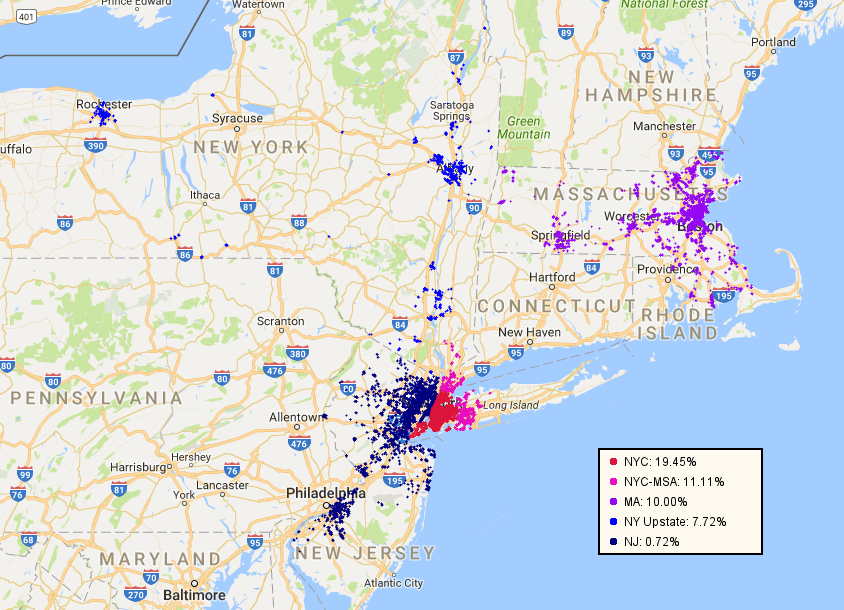
\includegraphics[width=6in]{full_yelp_map.png}

{\footnotesize \raggedright \underline{Notes:} Each data point represents a restaurant in the Yelp dataset. Samples are color coded by the magnitude of the increase in minimum wage on January 1, 2017. NYC saw the highest increase in minimum wage at 19.45\%. NYC-MSA, which includes Nassau, Suffolk, and Westchester counties, saw the second highest increase at 11.11\%. The minimum wage increased in MA by 10.00\%, in Upstate NY by 7.72\% and in NJ by 0.72\%. \par}
\end{figure}

\vspace*{\fill}


\newpage

\vspace*{\fill}


\begin{figure}[H]
\centering
\caption{Geographic Location of Restuarants Used in Border Effects Analysis}
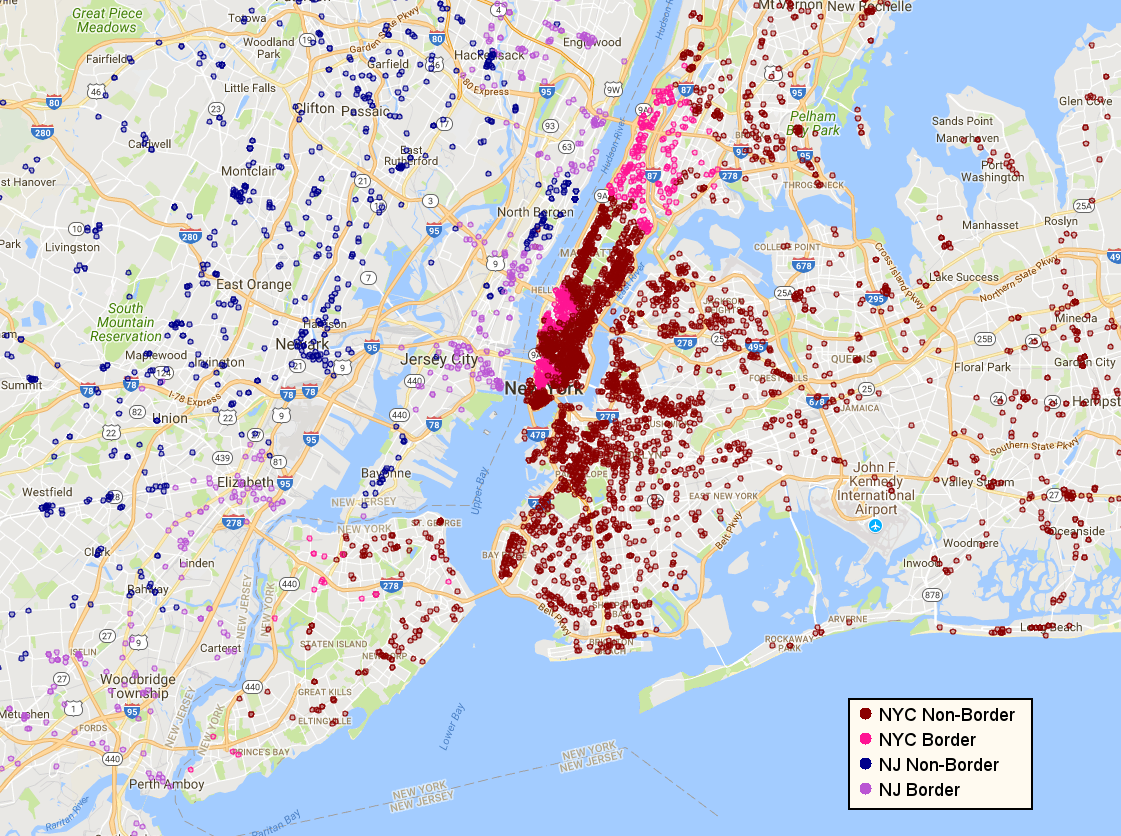
\includegraphics[width=6in]{border.png}

{\footnotesize \raggedright \underline{Notes:} Each data point represents a restaurant in the Yelp dataset in NJ and NYC. Samples are color coded by the magnitude of the increase in minimum wage on January 1, 2017, and use in the border effects analysis. The highlighted restaurants in each group represent the restaurants that are within twelve minutes from the border and are used in the border effects analysis. \par
}
\end{figure}

\vspace*{\fill}

\newpage

\vspace*{\fill}


\begin{figure}[H]
\centering
\caption{Quality Changes by Initial Quality Rating}
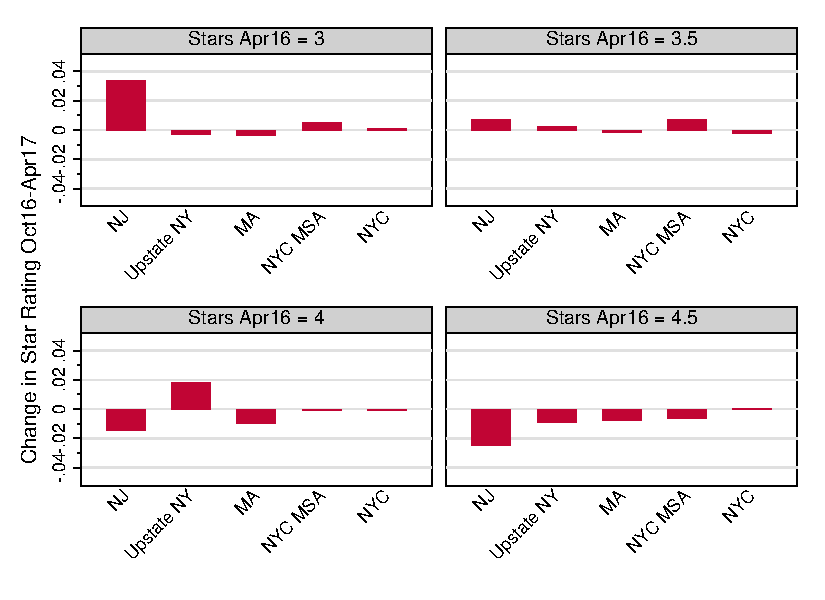
\includegraphics[width=5in]{qualitybars.pdf}

{\footnotesize \raggedright \underline{Notes:} The figures show the relationship between the change in star rating from October 2016 to April 2017 and the change in minimum wage by initial quality rating. The minimum wage groups are reported in ascending order with respect to the increase in minimum wage that occurred in January 2017. The initial star value is the Yelp consumer rating of the restaurants in April 2016. Change in star rating is reported as percentage change. All restaurants that have a star rating throughout the dataset are included in the plots.   \par}
\end{figure}


\vspace*{\fill}


\newpage

\vspace*{\fill}


\begin{figure}[H]
\centering
\caption{Border Effects:  Price Pass Through by Distance to NYC/NJ Border}
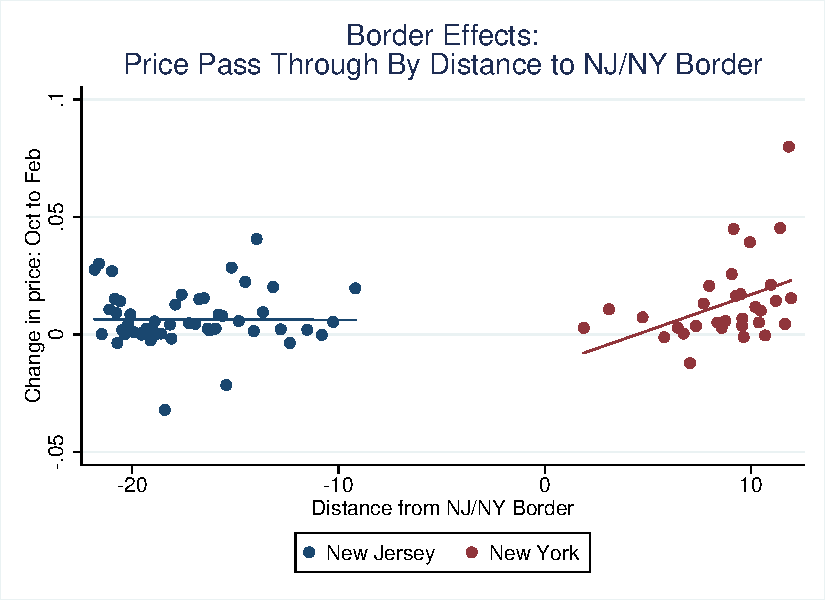
\includegraphics[scale=.75]{gh_dist.pdf}

{\footnotesize \raggedright \underline{Notes:} The figure shows the relationship between the change in price from October 2016 to April 2017 and the distance to the NYC- NJ border. Restaurants are binned into 80 quantiles. There is a gap between the NYC and NJ restaurants due to the Hudson River which separates the two states. Distance is measured in driving minutes to the nearest restaurant on the opposite side of the border. \par }

\end{figure}
%

\vspace*{\fill}


\newpage 

\section{Tables}

\vspace*{\fill}


\begin{table}[H]
\centering
\caption{Minimum Wage Policy Changes}
\begin{tabularx}{1\textwidth}{ l*{1}{Y} c *{6}{Y} } \\ \hline 
%\begin{tabular}{ cccccc } \\ \hline 
 & \multicolumn{3}{c}{Regular Minimum Wage} & \multicolumn{3}{c}{Tipped Minimum Wage}\\
 Area & `16  & `17  & $\% \Delta$ & `16 & `17 &  $\% \Delta$  \\ \hline 
%&&& \\
%1 &  NYC \& FF & \$10.50 & \$12.00 & 14.29\%& - & - & - \\
 %2 & NY Upstate \& FF  & \$9.75 & \$10.75 & 10.26\% & - & -& - \\
 NYC \& Lg & \$9.00 & \$11.00 & 22.22\% & \$7.50 & \$7.50 & 0.00\%\\
 NYC \& Sm & \$9.00 & \$10.50 & 16.67 \% & \$7.50 & \$7.50 & 0.00\%\\
 NYC MSA & \$9.00 & \$10.00 & 11.11\% & \$7.50 & \$7.50 & 0.00\%\\
NY Upstate & \$9.00 & \$9.70 & 7.78\% & \$7.50 & \$7.50  & 0.00\% \\
%7 & Connecticut & \$9.60 & \$10.10 & 5.21\% & \$6.07 & \$6.38 & 5.11\% \\
 New Jersey &  \$8.38 & \$8.44 & 0.72\%  & \$2.13 & \$2.3 & 0.00\% \\
 Massachusetts & \$10.00 & \$11.00 & 10.00\% & \$3.00 & \$3.75  & 25.00\% \\ \hline
%10 & Pennsylvania &  \$7.25 & \$7.25 & 0.00\% & \$2.83 & \$2.83 & 0.00\% \\
%11 & Vermont &  \$9.60 & \$10.00 & 4.2\% & \$4.80 & \$5.00 & 4.2\% \\
\end{tabularx}
%\end{tabular}

\bigskip


{\footnotesize \raggedright \underline{Notes:} The regular and tipped minimum wage changes from 2016 to 2017 are reported by group. The first two rows show the minimum wage changes for restaurants in NYC. A small restaurant is defined as having 10 employees or less, and a large restaurant is defined by more than 10 employees. For the main analysis I use the average of the two minimum wage changes, 19.45\%, for both small and large restaurants in NYC. The NYC MSA group consists of restaurants in the three contiguous counties to NYC: Nassau, Suffolk, and Westchester. NY Upstate encapsulates restaurants in all other areas of the state. NJ and MA minimum wage laws are consistent throughout each state.  \par }
\end{table}

\vspace*{\fill}



\begin{table}[p]
\centering
\caption{Yelp Restaurant Summary Statistics by Minimum Wage Group}
\begin{center}
\begin{tabular}{lccccc}
\hline  & (1) & (2) & (3) & (4) & (5)\\
 & NYC & NYC MSA & MA & NY Upstate & NJ\\
\hline  \textit{Min Wage Increase}  & 0.194 & 0.111 & 0.100 & 0.078 & 0.007\\
  & (0.000) & (0.000) & (0.000) & (0.000) & (0.000)\\
 \textit{Starting Price (Apr16)}  & 9.781 & 10.703 & 9.891 & 9.622 & 9.869\\
  & (7.030) & (6.545) & (5.541) & (8.544) & (7.737)\\
 \textit{Number of Items}  & 60.462 & 78.084 & 67.136 & 62.193 & 73.419\\
  & (80.136) & (82.284) & (76.173) & (72.106) & (90.365)\\
 \textit{Change Price (Apr16-Oct16)}  & 0.005 & 0.002 & 0.003 & 0.003 & 0.005\\
  & (0.048) & (0.060) & (0.057) & (0.033) & (0.044)\\
 \textit{Change Price (Oct16-Apr17)}  & 0.008 & 0.007 & 0.005 & 0.001 & 0.004\\
  & (0.070) & (0.088) & (0.053) & (0.019) & (0.073)\\
 \textit{Increase}  & 0.145 & 0.089 & 0.115 & 0.040 & 0.085\\
  & (0.353) & (0.285) & (0.319) & (0.197) & (0.280)\\
 \textit{Decrease}  & 0.041 & 0.025 & 0.028 & 0.015 & 0.032\\
  & (0.199) & (0.157) & (0.164) & (0.123) & (0.177)\\
 \textit{Price Change $\|$ Increase}  & 0.083 & 0.108 & 0.064 & 0.048 & 0.087\\
  & (0.110) & (0.260) & (0.125) & (0.065) & (0.215)\\
 \textit{Price Change $\|$ Decrease}  & -0.100 & -0.089 & -0.097 & -0.048 & -0.095\\
  & (0.210) & (0.157) & (0.100) & (0.063) & (0.118)\\
 \textit{Sales (100k)}  & 8.489 & 7.597 & 9.233 & 5.019 & 5.631\\
  & (14.245) & (37.176) & (19.165) & (5.988) & (9.583)\\
 \textit{Employees} & 10.836 & 10.227 & 14.603 & 10.222 & 9.267\\
  & (15.415) & (20.926) & (24.594) & (11.832) & (15.260)\\
 \textit{Limited Service}  & 0.042 & 0.072 & 0.019 & 0.069 & 0.043\\
  & (0.201) & (0.258) & (0.135) & (0.254) & (0.202)\\
 \textit{Franchise}  & 0.001 & 0.006 & 0.016 & 0.000 & 0.010\\
  & (0.029) & (0.077) & (0.126) & (0.000) & (0.097)\\
\hline  $ N $  & 4242 & 595 & 1658 & 519 & 1793\\
\hline\end{tabular}\\
\end{center}

{\footnotesize \raggedright \underline{Notes:} The means and standard deviations of the primary dataset, Yelp, are reported. Each column contains the restaurants that fall into a specific minimum wage group. All data is balanced at the item level across time periods and aggregated at the restaurant level. The fourth and fifth rows report mean change in natural log of the price, which is approximately the percentage change. The rows titled ``Increase'' and ``Decrease'' report the percentage of restaurants that increased or decreased price between Oct `16 and Apr '17. The conditional price changes are calculated from Oct `16 to Apr '17. \par }
\end{table}





\begin{table}[p]
\centering
\caption{Grubhub Restaurant Summary Statistics by Minimum Wage Group}
\begin{center}
\begin{tabular}{lccccc}
\hline  & (1) & (2) & (3) & (4) & (5)\\
 & NYC & NYC MSA & MA & NY Upstate & NJ\\
\hline  \textit{Min Wage Increase}  & 0.194 & 0.111 & 0.100 & 0.078 & 0.007\\
  & (0.000) & (0.000) & (0.000) & (0.000) & (0.000)\\
 \textit{Starting Price (Dec16)}  & 9.356 & 9.759 & 9.346 & 8.640 & 8.949\\
  & (5.589) & (3.513) & (4.182) & (2.787) & (3.761)\\
 \textit{Number of Items}  & 107.790 & 133.704 & 117.472 & 105.053 & 126.917\\
  & (89.516) & (87.262) & (73.827) & (74.815) & (87.014)\\
 \textit{Change Price (Dec16-Apr17)}  & 0.013 & 0.008 & 0.009 & 0.013 & 0.006\\
  & (0.044) & (0.027) & (0.036) & (0.036) & (0.034)\\
 \textit{Increase}  & 0.374 & 0.326 & 0.294 & 0.349 & 0.292\\
  & (0.484) & (0.469) & (0.456) & (0.477) & (0.455)\\
 \textit{Decrease}  & 0.066 & 0.060 & 0.053 & 0.047 & 0.073\\
  & (0.249) & (0.238) & (0.224) & (0.213) & (0.260)\\
 \textit{Price Change $\|$ Increase}  & 0.040 & 0.027 & 0.035 & 0.037 & 0.029\\
  & (0.054) & (0.034) & (0.049) & (0.051) & (0.041)\\
 \textit{Price Change $\|$ Decrease}  & -0.025 & -0.019 & -0.030 & -0.011 & -0.026\\
  & (0.076) & (0.054) & (0.068) & (0.019) & (0.075)\\
 \textit{Sales (100k)}  & 8.643 & 3.218 & 4.976 & 4.684 & 2.987\\
  & (42.233) & (4.072) & (7.722) & (6.363) & (3.007)\\
 \textit{Employees} & 9.916 & 5.650 & 7.996 & 9.582 & 5.130\\
  & (18.763) & (7.000) & (12.253) & (13.502) & (5.172)\\
 \textit{Limited Service}  & 0.042 & 0.070 & 0.029 & 0.067 & 0.065\\
  & (0.202) & (0.255) & (0.168) & (0.251) & (0.247)\\
 \textit{Franchise}  & 0.004 & 0.007 & 0.011 & 0.021 & 0.000\\
  & (0.064) & (0.083) & (0.105) & (0.142) & (0.000)\\
\hline  $ N $  & 4172 & 565 & 866 & 358 & 1320\\
\hline\end{tabular}\\
\end{center}

{\footnotesize \raggedright \underline{Notes:}  The means of the secondary dataset, Grubhub, are reported.  Each column contains the restaurants that fall into a specific minimum wage group. All data is balanced at the item level across time periods and aggregated at the restaurant level. The fourth row reports mean change in natural log of the price, which is approximately the percentage change. The rows titled ``Increase'' and ``Decrease'' report the percentage of restaurants that increased or decreased the averaged menu item price between Dec `16 and Apr `17. The conditional price changes calculated from Dec `16 to Apr `17. \par
}
\end{table}



\newpage

%\begin{landscape}
\begin{table}
\centering
\caption{Main Price Pass Through Results}
<<<<<<< HEAD
\begin{center}
\begin{tabular}{lccccc}
\hline  & \multicolumn{3}{c}{Yelp} & \multicolumn{2}{c}{Grubhub}\\
 & (1) & (2) & (3) & (4) & (5)\\
 & All & Cntrls & Change & All & Cntrls\\
\hline  $ Apr16-Jul16 $  & -0.019 & 0.053 & -0.149 &  & \\
 & (0.062) & (0.114) & (0.374) &  & \\
 $ Jul16-Oct16 $  & 0.069 & 0.063 & 0.262 &  & \\
 & (0.080) & (0.120) & (0.409) &  & \\
 $ Oct16-Jan17 $  & 0.163 & 0.208 & 0.604 &  & \\
 & (0.056) & (0.083) & (0.317) &  & \\
 $ Jan17-Apr17 $  & 0.150 & 0.180 & 0.464 &  & \\
 & (0.060) & (0.096) & (0.353) &  & \\
\hline  $ Dec16-Jan17 $  &  &  &  & 0.254 & 0.272\\
 &  &  &  & (0.002) & (0.010)\\
 $ Jan17-Feb17 $  &  &  &  & 0.233 & 0.331\\
 &  &  &  & (0.016) & (0.040)\\
 $ Feb17-Mar17 $  &  &  &  & 0.188 & 0.246\\
 &  &  &  & (0.021) & (0.015)\\
 $ Mar17-Apr17 $  &  &  &  & 0.171 & 0.165\\
 &  &  &  & (0.008) & (0.020)\\
\hline \textit{Total Pass Through} & 0.313 & 0.388 & 1.068 & 0.845 & 1.015$^+$\\
  & (0.115) & (0.171) & (0.669) & (0.031) & (0.083)\\
\hline  $ N $  & 8805 & 5257 & 2099 & 7280 & 3230\\
 $ NxT $  & 35220 & 21028 & 8396 & 29120 & 12920\\
\hline\end{tabular}\\
\begin{tiny}+ statistically different than respective 'All' column \end{tiny}\\
\end{center}
=======
\begin{center}
\begin{tabular}{lccccc}
\hline  & \multicolumn{3}{c}{Yelp} & \multicolumn{2}{c}{Grubhub}\\
 & (1) & (2) & (3) & (4) & (5)\\
 & All & Cntrls & Change & All & Cntrls\\
\hline  $ Apr16-Jul16 $  & -0.019 & 0.053 & -0.149 &  & \\
 & (0.062) & (0.114) & (0.374) &  & \\
 $ Jul16-Oct16 $  & 0.069 & 0.063 & 0.262 &  & \\
 & (0.080) & (0.120) & (0.409) &  & \\
 $ Oct16-Jan17 $  & 0.163 & 0.208 & 0.604 &  & \\
 & (0.056) & (0.083) & (0.317) &  & \\
 $ Jan17-Apr17 $  & 0.150 & 0.180 & 0.464 &  & \\
 & (0.060) & (0.096) & (0.353) &  & \\
\hline  $ Dec16-Jan17 $  &  &  &  & 0.254 & 0.272\\
 &  &  &  & (0.002) & (0.010)\\
 $ Jan17-Feb17 $  &  &  &  & 0.233 & 0.331\\
 &  &  &  & (0.016) & (0.040)\\
 $ Feb17-Mar17 $  &  &  &  & 0.188 & 0.246\\
 &  &  &  & (0.021) & (0.015)\\
 $ Mar17-Apr17 $  &  &  &  & 0.171 & 0.165\\
 &  &  &  & (0.008) & (0.020)\\
\hline \textit{Total Pass Through} & 0.313 & 0.388 & 1.068 & 0.845 & 1.015$^+$\\
  & (0.115) & (0.171) & (0.669) & (0.031) & (0.083)\\
\hline  $ N $  & 8805 & 5257 & 2099 & 7280 & 3230\\
 $ NxT $  & 35220 & 21028 & 8396 & 29120 & 12920\\
\hline\end{tabular}\\
\begin{tiny}+ statistically different than respective 'All' column \end{tiny}\\
\end{center}
>>>>>>> 9bf80c4d3367c601bceb3268e37dc31cf9116a6c


{\footnotesize \raggedright \underline{Notes:}  
The outcome variable for all columns is the log change in price at the restaurant level. All standard errors are clustered at the minimum wage group level. Each row represents the amount of pass-through occurring in the lag(s), lead(s), and contemporaneous time periods of the minimum wage changes. For the specifications using the Yelp data, (1)-(3), the total pass-through estimates are linear combinations of the October '16 to January '17 and the January '17 to April '17 estimates. For the specifications using the Grubhub data, (4)-(5), all time periods are included in the total pass-through estimates. The first column includes the full Yelp sample. The second column includes the vector of controls from the RUSA dataset, comprised of sales volume, number of employees and limited service status. The third column includes only restaurants that changed at least one item over the time period of the dataset. Column 4 reports price pass-through estimates using the full Grubhub sample. Column 5 includes the vector of RUSA control variables.   \par
}
\end{table}
%\end{landscape}



\begin{table}
\centering
\caption{Price Pass Through By Restaurant Characteristics}
\begin{center}
\begin{tabular}{lcccccc}
\hline  & (1) & (2) & (3) & (4) & (5) & (6)\\
 & Low Sales & High Sales & Low Emps & High Emps & Low Stars & High Stars\\
\hline  $ Apr16-Jul16 $  & 0.288 & 0.182 & 0.249 & 0.122 & 0.189 & 0.026\\
 & (0.145) & (0.271) & (0.147) & (0.260) & (0.076) & (0.114)\\
 $ Jul16-Oct16 $  & 0.249 & -0.073 & 0.286 & 0.019 & 0.260 & 0.153\\
 & (0.182) & (0.204) & (0.140) & (0.245) & (0.056) & (0.126)\\
 $ Oct16-Jan17 $  & 0.260 & 0.096 & 0.364 & 0.032 & 0.429 & 0.189\\
 & (0.126) & (0.121) & (0.119) & (0.155) & (0.033) & (0.080)\\
 $ Jan16-Apr17 $  & 0.468 & 0.334 & 0.238 & 0.386 & 0.361 & 0.190\\
 & (0.122) & (0.142) & (0.132) & (0.176) & (0.094) & (0.103)\\
\hline \textit{Total Pass Through} & 0.728 & 0.43 & 0.602$^+$ & 0.418$^+$ & 0.79 & 0.379\\
  & (0.244) & (0.262) & (0.231) & (0.331) & (0.119) & (0.183)\\
\hline  $ N $  & 1556 & 1723 & 2142 & 1894 & 3832 & 6783\\
 $ NxT $  & 6224 & 6892 & 8568 & 7576 & 15328 & 27132\\
\hline\end{tabular}\\
\begin{tiny} + statistically different than comparison group \end{tiny}\\
\end{center}

{\footnotesize \raggedright \underline{Notes:} 
The reported values compare price pass-through of restaurants in the lowest and highest third based on sales, employees, and number of stars in April 2016 using the Yelp dataset. The outcome variable for all columns is the log change in price at the restaurant level. All standard errors are clustered at the minimum wage group level. The total pass-through estimates are linear combinations of the October '16 to January '17 and the January '17 to April '17 estimates.  The cutoff values for sales are 204 and 598 thousand. The cutoff values for employees are 4 and 10, and the cutoff values for stars are 3 and 4. \par
}
\end{table}

\begin{landscape}
\begin{table}
\centering
\caption{Price Pass Through By Item Type}
\begin{center}
\begin{tabular}{lcccccccc}
\hline  & (1) & (2) & (3) & (4) & (5) & (6) & (7) & (8)\\
 & All & Popular & Side & Sandwich & Soup/Salad & Entre & Dessert & Drink\\
\hline  $ Dec16-Jan17 $  & 0.155 & 0.193 & 0.169 & 0.224 & 0.174 & 0.117 & 0.114 & 0.146\\
 & (0.004) & (0.002) & (0.008) & (0.004) & (0.002) & (0.002) & (0.009) & (0.005)\\
 $ Jan17-Feb17 $  & 0.142 & 0.238 & 0.163 & 0.244 & 0.132 & 0.121 & 0.078 & 0.152\\
 & (0.013) & (0.007) & (0.054) & (0.008) & (0.008) & (0.007) & (0.024) & (0.027)\\
 $ Feb17-Mar17 $  & 0.126 & 0.072 & 0.208 & 0.180 & 0.109 & 0.087 & 0.141 & 0.067\\
 & (0.010) & (0.015) & (0.029) & (0.005) & (0.009) & (0.009) & (0.021) & (0.023)\\
 $ Mar17-Apr17 $  & 0.060 & 0.084 & 0.115 & 0.070 & 0.099 & 0.050 & 0.041 & 0.015\\
 & (0.012) & (0.010) & (0.028) & (0.038) & (0.015) & (0.015) & (0.024) & (0.014)\\
\hline \textit{Total Pass Through} & 0.483 & 0.587$^+$ & 0.656$^+$ & 0.718$^+$ & 0.514 & 0.375$^+$ & 0.373 & 0.379$^+$\\
  & (0.032) & (0.023) & (0.104) & (0.045) & (0.022) & (0.026) & (0.076) & (0.054)\\
\hline  $ N $  & 831763 & 47295 & 107172 & 105265 & 46692 & 150035 & 18453 & 65112\\
 $ NxT $  & 3327052 & 189180 & 428688 & 421060 & 186768 & 600140 & 73812 & 260448\\
\hline\end{tabular}\\
\begin{tiny} + statistically different than column (1)\end{tiny}\\
\end{center}

{\footnotesize \raggedright \underline{Notes:} 
The outcome variable for all columns is the log change in price at the item level using the Grubhub dataset. All standard errors are clustered at the minimum wage group level. All time periods are included in the total pass-through estimates. The item categories listed above are mutually exclusive but not exhaustive. The additional food categories not listed include; Appetizer, Kids, Pizza, and Other. \par
}
\end{table}
\end{landscape}

\newpage 

\vspace*{\fill}
%\begin{landscape}
\begin{table}[H]
\centering
\caption{Overall Yelp Quality Changes by Initial Star Rating}
<<<<<<< HEAD
\begin{center}
\begin{tabular}{lcccccc}
\hline  & (1) & (2) & (3) & (4) & (5) & (6)\\
 & All &  $ 2.5 $  &  $ 3.0 $  &  $ 3.5 $  &  $ 4.0 $  &  $ 4.5$ \\
\hline  $ Apr16-Jul16 $  & 0.035 & 1.138 & 0.625 & 0.068 & -1.047 & -0.627\\
 & (0.213) & (1.201) & (0.697) & (0.187) & (0.312) & (0.456)\\
 $ Jul16-Oct16 $  & -0.046 & -0.321 & -0.305 & 0.109 & 0.198 & -0.792\\
 & (0.071) & (0.292) & (0.400) & (0.211) & (0.296) & (0.413)\\
 $ Oct16-Jan17 $  & 0.049 & 0.255 & -1.341 & -0.268 & 0.500 & 0.470\\
 & (0.036) & (1.068) & (0.178) & (0.076) & (0.090) & (0.275)\\
 $ Jan17-Apr17 $  & -0.416 & -1.158 & -0.546 & -0.728 & -0.252 & -0.255\\
 & (0.167) & (0.609) & (0.670) & (0.197) & (0.080) & (0.175)\\
\hline \textit{Total \% Change Stars} & -0.368 & -0.903 & -1.887 & -0.996 & 0.248 & 0.215\\
  & (0.138) & (1.667) & (0.813) & (0.161) & (0.123) & (0.164)\\
\hline  $ N $  & 6392 & 625 & 1080 & 1801 & 1904 & 982\\
 $ NxT $  & 25568 & 2500 & 4320 & 7204 & 7616 & 3928\\
\hline\end{tabular}\\
\begin{tiny} \hfil\end{tiny}\\
\end{center}
=======
\begin{center}
\begin{tabular}{lcccccc}
\hline  & (1) & (2) & (3) & (4) & (5) & (6)\\
 & All &  $ 2.5 $  &  $ 3.0 $  &  $ 3.5 $  &  $ 4.0 $  &  $ 4.5$ \\
\hline  $ Apr16-Jul16 $  & 0.035 & 1.138 & 0.625 & 0.068 & -1.047 & -0.627\\
 & (0.213) & (1.201) & (0.697) & (0.187) & (0.312) & (0.456)\\
 $ Jul16-Oct16 $  & -0.046 & -0.321 & -0.305 & 0.109 & 0.198 & -0.792\\
 & (0.071) & (0.292) & (0.400) & (0.211) & (0.296) & (0.413)\\
 $ Oct16-Jan17 $  & 0.049 & 0.255 & -1.341 & -0.268 & 0.500 & 0.470\\
 & (0.036) & (1.068) & (0.178) & (0.076) & (0.090) & (0.275)\\
 $ Jan17-Apr17 $  & -0.416 & -1.158 & -0.546 & -0.728 & -0.252 & -0.255\\
 & (0.167) & (0.609) & (0.670) & (0.197) & (0.080) & (0.175)\\
\hline \textit{Total \% Change Stars} & -0.368 & -0.903 & -1.887 & -0.996 & 0.248 & 0.215\\
  & (0.138) & (1.667) & (0.813) & (0.161) & (0.123) & (0.164)\\
\hline  $ N $  & 6392 & 625 & 1080 & 1801 & 1904 & 982\\
 $ NxT $  & 25568 & 2500 & 4320 & 7204 & 7616 & 3928\\
\hline\end{tabular}\\
\begin{tiny} \hfil\end{tiny}\\
\end{center}
>>>>>>> 9bf80c4d3367c601bceb3268e37dc31cf9116a6c

{\footnotesize \raggedright \underline{Notes:} 
The outcome variable for all columns is the log change in Yelp star rating. All standard errors are clustered at the minimum wage group level. The total percent change in stars estimates are linear combinations of the October '16 to January '17 and the January '17 to April '17 estimates. The initial star ratings are the rounded Yelp star ratings in April '16. Restaurants below a 2.5 rating and above a 4.5 rating are not analyzed as subsamples given that they are close to the lower and upper bounds, respectively, and so only have one direction to move. \par
}
\end{table}
%\end{landscape}
\vspace*{\fill}

\newpage 

\vspace*{\fill}

\begin{table}[H]\caption{Grubhub Food Specific Quality Changes by Initial Quality Rating}
<<<<<<< HEAD
\begin{center}
\begin{tabular}{lccc}
\hline  & (1) & (2) & (3)\\
 & All &  $<=$ Median  &  $>$ Median\\
\hline  $ Dec16-Jan17 $  & -0.069 & -0.349 & 0.156\\
 & (0.061) & (0.181) & (0.052)\\
 $ Jan17-Feb17 $  & -0.023 & -0.210 & 0.136\\
 & (0.102) & (0.169) & (0.049)\\
 $ Feb17-Mar17 $  & -0.171 & -0.317 & -0.018\\
 & (0.045) & (0.051) & (0.037)\\
 $ Mar17-Apr17 $  & -0.054 & -0.176 & 0.048\\
 & (0.019) & (0.056) & (0.066)\\
\hline \textit{Total \% Change Rating} & -0.316 & -1.215 & 0.344\\
  & (0.000) & (0.003) & (0.004)\\
\hline  $ N $  & 7281 & 3979 & 3302\\
 $ NxT $  & 29124 & 15916 & 13208\\
\hline\end{tabular}\\
\begin{tiny} \hfil\end{tiny}\\
\end{center}
=======
\begin{center}
\begin{tabular}{lccc}
\hline  & (1) & (2) & (3)\\
 & All &  $<=$ Median  &  $>$ Median\\
\hline  $ Dec16-Jan17 $  & -0.069 & -0.349 & 0.156\\
 & (0.061) & (0.181) & (0.052)\\
 $ Jan17-Feb17 $  & -0.023 & -0.210 & 0.136\\
 & (0.102) & (0.169) & (0.049)\\
 $ Feb17-Mar17 $  & -0.171 & -0.317 & -0.018\\
 & (0.045) & (0.051) & (0.037)\\
 $ Mar17-Apr17 $  & -0.054 & -0.176 & 0.048\\
 & (0.019) & (0.056) & (0.066)\\
\hline \textit{Total \% Change Rating} & -0.316 & -1.215 & 0.344\\
  & (0.000) & (0.003) & (0.004)\\
\hline  $ N $  & 7281 & 3979 & 3302\\
 $ NxT $  & 29124 & 15916 & 13208\\
\hline\end{tabular}\\
\begin{tiny} \hfil\end{tiny}\\
\end{center}
>>>>>>> 9bf80c4d3367c601bceb3268e37dc31cf9116a6c

{\footnotesize \raggedright \underline{Notes:} 
The outcome variable for all columns is the log change in Grubhub Food Quality rating. The food specific quality rating is on a 1 to 100 scale and represents the proportion of customers that reported that ``the food was good" after receiving their order. All standard errors are clustered at the minimum wage group level. The total percent change in rating estimates are linear combinations of all rows. The median food quality rating is 89. \par
}
\end{table}

\vspace*{\fill}


\vspace*{\fill}

% \vspace{100mm} 

\newpage 

\vspace*{\fill}
\begin{table}[H]
\centering
\caption{Border Effects}
\begin{center}
\begin{tabular}{lccc}
\hline Source & \multicolumn{2}{c}{Yelp} & Grubhub\\
 & (1) & (2) & (3)\\
Time Frame & Oct16-Apr17 & Apr16-Oct16 & Dec16-Apr17\\
\hline  $ \mathbbm{1}(NY) \quad (\alpha_1) $  & 0.0064 & -0.0064 & -0.0102\\
  & (0.0152) & (0.0116) & (0.0124)\\
 Distance $\quad (\alpha_2) $  & -0.0009 & 0.0000 & -0.0000\\
  & (0.0008) & (0.0006) & (0.0006)\\
 Distance * $ \mathbbm{1}(NY) \quad (\alpha_3) $  & 0.0020 & 0.0007 & 0.0019\\
  & (0.0011) & (0.0009) & (0.0009)\\
 Constant $\quad (\alpha_0) $  & -0.0069 & 0.0041 & 0.0059\\
  & (0.0134) & (0.0102) & (0.0101)\\
\hline  $ \alpha_2 + \alpha_3 $  & 0.0011 & 0.0007 & 0.0018\\
  & (0.0008) & (0.0006) & (0.0007)\\
\hline  $ N $  & 1002 & 1002 & 694\\
\hline\end{tabular}\\
\end{center}

{\footnotesize \raggedright \underline{Notes:} 
The outcome variable is the percentage point change in price due to a 10 minute change in the distance of a restaurant to the border. The first column includes restaurants in the Yelp dataset within twelve minutes of the NYC - NJ border between October 2016 and April 2017. Column 2 includes these same restaurants but using the change in price from July 2016 to October 2016 as the outcome. Column 3 reports effects on the NYC-NJ border using the Grubhub dataset. \par
}
\end{table}
\vspace*{\fill}

%
%\section{Appendix}
%
%\subsection{Data Collection}
%
%\subsection{Variable Definitions}
%






\end{document}












=======
\documentclass[11pt]{article}

\usepackage{blindtext}
\usepackage[pdftex]{graphicx}
\usepackage{fancyhdr}
\usepackage[margin=.8in]{geometry}
\usepackage[hang]{footmisc}
\usepackage{lipsum}
 \usepackage[flushleft]{threeparttable}
 \usepackage{tabularx} 
\usepackage{apacite}
\usepackage{float}
\usepackage{caption}
\usepackage{subcaption}
\usepackage{amsmath}
%\pagestyle{headings}
%\fancyhf{}
%\rhead{djfklas}
%\lhead{dkjfalj}
%\rfoot{ Page \thepage}
\usepackage{breqn}
\usepackage{titlesec}
\usepackage[labelfont={bf}]{caption}
%\usepackage{hyperref}
\usepackage{setspace}
\interfootnotelinepenalty=10000
\usepackage{arydshln}
\usepackage{rotating}
\usepackage{amsfonts}
\usepackage{bbm}
\usepackage{changepage}
\usepackage{pdflscape}
\newcommand{\etal}{\textit{et al}. }
\doublespacing
\newcolumntype{Y}{>{\centering\arraybackslash}X}

\def\sym#1{\ifmmode^{#1}\else\(^{#1}\)\fi}

\rfoot{ Page \thepage}
%
%\titleformat{\section}
%  {}{\thesection}{1em}{\textbf}
%  
% \titleformat{\subsection}
%  {\scshape}{\thesubsection}{1em}{\textbf}
%  
%  
%  \titleformat{\subsubsection}
%  {\scshape}{\thesubsubsection}{1em}{\textbf}
  
\newcommand\blfootnote[1]{%
  \begingroup
  \renewcommand\thefootnote{}\footnote{#1}%
  \addtocounter{footnote}{-1}%
  \endgroup
}

\title{Effects of a  Minimum Wage Increase On Restaurants:  \\ Price Pass Through, Quality Changes, and Border Effects}
\author{Chelsea Crain \footnote{Department of Economics, University of Iowa, Iowa City, IA, 52242, \textit{Email: }chelsea-crain@uiowa.edu } \thanks{I thank David Frisvold, Julia Garlick, Nicolas Ziebarth, Michael Andrews, Lance Cundy, David Enocksson, Ryan Rudderham, and seminar participants at the University of Iowa for helpful suggestions. Research reported in this publication was supported by the National Institute Of Diabetes And Digestive
And Kidney Diseases of the National Institutes of Health under Award Number R01DK107686.
The content is solely the responsibility of the author and does not necessarily represent the official views of the National Institutes of Health.} \\ University of Iowa}

\begin{document}

\maketitle

\begin{abstract}
The stagnant federal minimum wage in the U.S. has spurred an unprecedented number of state, county, and citywide minimum wage laws. The high number and varying magnitudes of minimum wage increases combined with the growing online presence of restaurants provides a unique setting in which to analyze the effects of a minimum wage increase on restaurants' prices and quality. Using a novel dataset comprised of menu item and restaurant quality information from thousands of east coast establishments across three states, I estimate the effects of varying levels of minimum wage increases enacted at the start of 2017. I find that prices rise 0.3\% - 1.1\% in response to a 10\% increase in the minimum wage. These price pass-through effects are heterogeneous across restaurant characteristics and item type. Further, the magnitude of price pass-through is significantly lower for restaurants near the border of a minimum wage policy region, suggesting that local minimum wage policies negatively affect businesses on the borders. Finally, I find that customer-perceived quality of restaurants is positively related to increases in the minimum wage for restaurants with high rating levels prior to a minimum wage hike, but negatively related for restaurants with low rating levels. 


\end{abstract}



\underline{JEL Classifications:} J08, J3, H7, H32 

\underline{Keywords:} minimum wage, price pass-through, firm quality, border effects

\newpage

\section{Introduction}
The federal minimum wage in the United States has remained stagnant for almost a decade at \$7.25, which is over 30\% lower in real terms than the federal minimum wage in 1970. As a result of this stagnation, a significant number of states, counties and cities across the country have introduced or are considering introducing a local minimum wage. In 2012 there were only five city or county minimum wage laws across the country, but by the beginning of 2017 there were over 40 \cite{localmws}. The number of state level minimum wage laws has also increased, with 19 states raising their respective minimum wage at the beginning of 2017 \cite{epimw}. Despite the prevalence of such policies, there remains no clear consensus in the minimum wage literature about the total effects of a minimum wage increase. The unique nature of the datasets that I use in this paper allow for more extensive analysis of minimum wage related questions. These additional areas of study include heterogeneity in price pass-through across restaurant characteristics and item type, changes in restaurant quality, and the difference in pass-through for restaurants closer to the border of areas with a higher minimum wage. 

Nearly three-fifths of all workers paid at or below the minimum wage are employed in the service industry \cite{charsmw}, making restaurants an ideal sector in which to analyze the effects of a minimum wage increase on price and quality. The price of restaurant food has become an integral part of the American budget. In 2015, for the first time in history, Americans spent more money eating out at restaurants than they did on groceries \cite{usda}. 
%Although low income workers receive a higher income after minimum wage hikes, low income workers purchase more minimum wage produced goods \cite{macurdy2000increasing}. This suggests that changes in restaurant prices affect the relative purchasing power of low income workers more than the average customer. 
Price changes due to a minimum wage increase also have implications about the underlying employment structure of the restaurant industry. Card and Kruger (1994) found a small positive effect on employment and no effect on prices after an increase in the minimum wage\nocite{card1994minimum}. These findings contradicted the textbook model of competitive labor markets, a model which predicts an increase in output prices and a decrease in employment. In response to Card and Kruger (1994), many studies analyzed the existence of monopsony power in the labor market \cite{manning1995we, rebitzer1995consequences, burdett1998wage, bhaskar1999minimum}, as a monopsony model predicts an increase in employment and a decrease in prices. Neumark and Wascher (2006)\nocite{neumark2006minimum} in their survey of the literature conclude that the most rigorous and reliable studies have found significant price increases and small employment decreases. As Aaronson, French and MacDonald (2008) conclude\nocite{aaronson2008minimum}, the presence of significant increases in price in response to minimum wage increases is evidence against the prevalence of monopsony power in the labor market. It is therefore expected that an increase in minimum wage will lead to an increase in output prices.


In the literature, the magnitude of the price pass-through to consumers after a 10\% increase in minimum wage varies between 0.4\% and 1.5\%. The following are specific examples that are most closely related to this paper. Allegrotto and Reich (2015) use full online menus to analyze prices before and after a local minimum wage increase in San Jose, and find pass-through to be 0.58\%\nocite{allegretto2015local}. Aaronsen, French and MacDonald (2008) utilize the store level data that comprises the food away from home component of the Consumer Price Index. This data contains several bundles of food, usually the equivalent of a meal, at a variety of establishments across the country. Using variation in state and federal minimum wage changes, the authors estimate a price pass-through of 0.7\%\nocite{aaronson2008minimum}. Basker and Khan (2013) estimate price pass-through of 0.9\% for McDonald's Quarter Pounders and a Pizza Hut regular cheese pizza using state level variation in the minimum wage\nocite{basker2016does}. These estimates vary with the types of items and time period analyzed but show that restaurants consistently pass-through the increased labor costs in the form of higher output prices. 


In this paper, I examine restaurants in three contiguous states on the East coast that increased their respective minimum wages (though by differing magnitudes) on the first day of 2017. I examine the impact of the minimum wage changes using restaurant menus from Yelp.com and Grubhub.com. Using these datasets, I estimate the overall price pass-through at the restaurant level due to a 10\% increase in minimum wage to be between 0.3\% and 1.1\%, depending on the subsample analyzed. These estimates are consistent with previous findings in the literature as discussed above. Unlike traditional administrative or government datasets, the data used in this study provide granular restaurant and menu data at the item level in real time. Furthermore, these data provide additional variables of interest, such as measures of quality, that are not available in traditional datasets. Utilizing restaurant specific characteristics, 
%The novel datasets that I use in this study also provide specific restaurant and item characteristics that allow for analysis beyond overall price pass-through. 
I find that the magnitude of the price pass-through estimate is heterogeneous across restaurant characteristics, with small and low quality restaurants showing significantly higher pass-through. The magnitude of the price pass-through also varies at the item level, where items in categories such as Popular, Side and Sandwich show a pass-through level of over 0.6\%, but items in categories such as Drink and Entr\'e show significantly lower levels of pass-through, with estimates below 0.4\%. This suggests that studies which examine prices of only a few menu items may significantly under or over estimate price pass-through. 



In addition to prices, restaurant quality could also be expected to change as a result of a minimum wage increase. For example, decreases in overall restaurant quality after a minimum wage hike could come in the form of reduced portion sizes or decreased food quality. On the other hand, an increase in the minimum wage could improve service quality by acting as an efficiency wage. Restaurants could also substitute toward more productive workers by decreasing work hours for less productive employees, improving average service quality. This is the first paper to analyze changes in customer-perceived quality due to a change in minimum wage. Using the consumer rated star values from the Yelp review platform, I estimate the impact of a 10\% minimum wage increase on the customer rating of restaurants, finding a bimodal effect. %of an increase in the minimum wage on restaurants. 
Restaurants that were rated at the median (3.5) or below prior to the minimum wage increase saw a significant decrease in the star rating given to them by consumers, where restaurants that started at ratings above 3.5 stars saw a positive effect on their consumer ratings due to the increase in minimum wage. These results suggest that firms may react to a minimum wage increase differently depending on initial quality. A similar conclusion was drawn by Luca and Luca (2017), who used Yelp data to analyze the probability of restaurant closure after a minimum wage increase. The authors found that the 
%ability of firms to adjust to increases in the minimum wage differ based on firm quality
likelihood of exit after a minimum wage hike significantly increased for restaurants rated at 3.5, but had no significant impact on 5 star restaurants\nocite{luca2017survival}. To investigate potential mechanisms of these overall quality effects found in the Yelp data, I next analyze changes in the Grubhub food specific quality measure. I find that restaurants starting at or below the median food quality rating significantly decreased food quality after a minimum wage increase, but that restaurants starting above the median rating significantly increased food quality. These food specific quality results support the overall quality results found in the Yelp data and provide support for the potential underlying mechanisms of these quality changes due to a minimum wage increase.

%I perform sentiment analysis on the text of customer reviews, creating a service specific measure of quality. Using this rough measure, I estimate that restaurants rated above the mean for overall quality significantly improved service quality in relationship to an increase in the minimum wage. In addition, I find that restaurants rated at or below the mean of overall quality decreased service quality in relationship to and increase in the minimum wage, although this is imprecisely measured. These results support the potential mechanisms that a minimum wage may act as an efficiency wage for higher quality restaurants or that higher quality restaurants are able to substitute towards more productive workers. 

One potential negative effect of a minimum wage increase is the inability of restaurants close to the border of the city, county, or state to account for these increased input costs in the form of higher prices without losing business. Restaurants facing minimum wage increases close to a border where competitors on the opposite side of the border are not facing an increase in labor costs may keep prices lower in order to compete. These effects are referred to as border effects, and can be measured by the existence of a significant relationship between the distance a restaurant is to a bordering area with a different minimum wage increase and the magnitude of the price increase. The existence of border effects is crucial with regard to policy evaluation and fully understanding how local businesses are affected by changes in minimum wage policy. This paper provides the most comprehensive analysis on the existence of border effects to date in the literature. For restaurants located close to a bordering area that is facing a lower minimum wage hike, I find a significant relationship between a restaurant's proximity to the border and the level of price pass-through. Specifically, I estimate that a restaurant ten minutes farther away from the border increases prices by 0.2 percentage points more than a restaurant on the border. These border effects suggest that a local minimum wage increase impedes the ability of restaurants to fully pass-through prices to consumers due to the spatial proximity to competitors who are not facing an increase in minimum wage. 






\section{Minimum Wage Laws}
On January 1, 2017, three contiguous states on the east coast - Massachusetts, New Jersey, and New York- increased their minimum wage at differing magnitudes, with a variety of levels of increase within the state of New York. Table 1 reports the increases in minimum wage in these areas, which range from 0.72\% to 22.22\%. These states provide a useful setting for minimum wage analysis as they are in the same geographic region and have similar economic, demographic, and political characteristics. Each area faced the changes in minimum wage over the same time period. 

In April of 2016, New York (NY) became the second state, after California, to pass a law that would incrementally raise the minimum wage for all workers to \$15/hour.\footnote{In 2015, NY passed a minimum wage law only applicable to fast food restaurants, increasing the minimum wage each year for fast food workers \cite{nyff}. Due to the small sample size and unique nature of fast food restaurants in the data, I exclude all fast food restaurants from the analysis.} In this law, which applies to all non-fast food restaurants, the degree of the minimum wage increase is based on the type and location of the establishment \cite{nybill}. The first two rows of Table 1 report minimum wage changes for restaurants in New York City (NYC). Restaurants in NYC with more than ten employees, denoted as large restaurants, saw a 22.22\% increase from, \$9 to \$11 per hour. Small restaurants in NYC saw an increase of 16.67\%, from \$9 to \$10.50. The third column of Table 1 includes restaurants of all sizes in the three contiguous counties outside of NYC: Nassau, Suffolk, and Westchester. These three counties are referred to throughout this paper as NYC MSA. These restaurants saw a 11.11\% increase. The final NY group, NY Upstate, which includes restaurants of all sizes elsewhere in the state of NY, saw a 7.78\% increase, from \$9 to \$9.70.

Two states contiguous to NY saw changes in their own state-wide minimum wage laws on January 1, 2017. In 2014, Massachusetts (MA) passed a bill that increased the minimum wage by \$1 a year from 2015-2017. This bill increased the minimum wage on January 1, 2017 by 10.00\%, from \$10 to \$11. \cite{mabill}. In the spring of 2016, New Jersey (NJ) proposed a minimum wage law similar to that of NY that would have raised the minimum wage to \$10.10 per hour on January 1, 2017, and would put the state on track to a \$15 minimum wage. The bill passed through the House and the Senate, but in August of 2016, NJ governor Chris Christie vetoed the bill, stating ``...[this bill] fails to consider the capacity of businesses, especially small businesses, to absorb the substantially increased labor costs it will impose''\cite{njveto}. Thus, in 2017, NJ increased the state minimum wage by only 0.72\%, a yearly adjustment for inflation \cite{njbill}. %In Pennsylvania (PA), workers saw no increase in the minimum wage at the beginning of 2017, as the state stayed at the federal level of \$7.25 7 \cite{panobill}. However, PA governor Tom Wolf called for an increase of the minimum wage to \$12/hour in his state budget proposal in February 2017 \cite{govwolf}. If passed, this would increase the PA minimum wage by an unprecedented 65\%. 
The state of NJ is therefore a strong counterfactual to NY and MA due to the similar political sentiment of the elected officials in the state Congress shown by the attempts at increasing the minimum wage. 




\section{Data}

I use three primary datasets to understand the impact of increases in the minimum wage on restaurant prices and quality. The first, and most extensive, is a panel dataset comprised of restaurant menu and quality information from Yelp.com. The second is a supplementary panel dataset comprised of restaurant menu information from Grubhub.com. The third is a dataset providing detailed restaurant business information from ReferenceUSA. I utilize these datasets to determine the magnitude of price pass-through to consumers, how this pass-through varies by restaurant and item specific characteristics, and how the minimum wage impacted customer-perceived quality.

\subsection{Yelp}

Yelp.com is a website in which consumers can find restaurant information including customer reviews, hours of operation, price range, and full menus. Yelp was founded in 2004, and currently has an average of 72 million monthly visitors with over 115 million reviews written \cite{yelpstat}. Using a web scrape, I conducted the first wave of Yelp data collection in April 2016, the second wave in July 2016, and the third wave in October 2016. Two waves of data collection occurred after the minimum wage increases, in January 2017 and April 2017.\footnote{See the data appendix for further details about the data collection process.} I collected information from the homepage of 69,224 restaurants within NY, NJ, and MA. Of these, 21,688, or approximately one third of these restaurants provide a full menu on Yelp.\footnote{Some restaurants provide an external link to a menu, but since these menus are not formatted uniformly, the menu information cannot be correctly parsed and thus for the sake of this dataset these restaurants fall into the same category as those restaurants who do not provide an online menu. These externally formatted menus were hand entered for one round of the scrape, and baseline characteristics of these restaurants were not statistically different from the Yelp formatted menus. See the data appendix for the comparison table reporting these baseline characteristics.} In a similar study using online menus, Allegrotto and Reich (2015) also found that on average about one third of restaurants posted full online menus\nocite{allegretto2016local}. Some restaurants, primarily chain restaurants, provide a full menu but do not include location specific prices. Out of the restaurants that post full menus, 17,385 of them include location specific prices. In order to match each restaurant to a minimum wage group, 15,087 restaurants were matched by address to a county using the Census Geocoder. The 47 fast food restaurants were removed from the dataset. To create a balanced panel, the final sample used in the analysis contains the 8,805 restaurants that posted location specific prices in all waves of data collection. Reasons that a restaurant may have failed to be in all waves of data collection include closures, name changes, or discontinued use of a Yelp menu. 


%One concern with using Yelp data is the reliability and frequency with which the information for a restaurant is updated, as Yelp menus may be updated at the restaurant owner or manager's discretion. As a way to deal with this reliability issue, I take advantage of a food delivery service that is powered by Yelp, called Eat24. This service provides customers the ability to order food directly from the restaurant's Yelp menu page for delivery or pickup. The use of this service ensures that the menu items and prices are up to date since customers are ordering directly from the provided menu information. Each restaurant in the dataset has an indicator for whether or not the business utilizes the Eat24 food delivery service. 

Yelp users provide online reviews of restaurants and assign them an overall star rating on a scale of 1 to 5, with 1 representing extremely poor and 5 representing outstanding. Although the number of stars that a restaurant has earned is determined by self-selected reviewers, the Yelp star rating has been found to be a reliable predictor of actual quality as well as an important determinant of profit for restaurants. In a study comparing Yelp star ratings of hospitals to an industry standard assessment of quality, Bardach \etal (2014) found that Yelp stars were significantly related to patient care and health outcomes\nocite{bardach2012relationship}. Luca (2011) used a regression-discontinuity design to analyze the impact of a change in the Yelp star rating on restaurants, and found that a one-star increase in the Yelp rating led to a 5-9\% increase in revenue\nocite{luca2011reviews}. A concern of using Yelp stars as a point of analysis regards restaurants writing fake reviews-- good reviews of themselves and bad reviews of competitors. Yelp uses a proprietary algorithm in an attempt to filter out fake reviews, which are not included in the Yelp star rating. Although some fake reviews may still exist, it is unlikely that any fake reviews on quality are correlated with changes in the minimum wage. The rounded star rating that customers see prominently displayed on each restaurant's homepage is the monthly average of all Yelp reviews rounded to the nearest half star.\footnote{If a restaurant has less than 10 reviews within a month, then the most recent reviews are added until the sample size reaches 10.} There is significant variation in the Yelp star rating for restaurants over the time period of the dataset, an indication that Yelp users are active in reporting the current quality of the establishments. Over 50 percent of restaurants see a change in star rating between any given observation period, and the average change given an increase (decrease) is 0.62 (0.61) stars. 

% As a second measure of quality, I perform sentiment analysis on the text of customer reviews, identifying positive and negative reviews that are specifically about service quality.\footnote{I use Python's Natural Language Toolkit for all sentiment analysis. More details of this analysis are available in the Data Appendix.} The program first identifies sentences where the subject is a service related entity (waiter, staff, hostess, etc.). Then based on a list of over 100 postive and negative adjectives that I provide to the program (helpful, nice, attentive, rude, careless, etc), classifies the sentence based on the service related adjective and adverb. I perform this sentiment analysis on all reviews for each restaurant, creating variables that identify the number of positive reviews on service and the number of negative reviews on service for each restaurant within each quarter between data collection waves. The majority of customer reviews contain general statements about a restaurant that are not specific to service quality, and therefore are not included in this measure.   


\subsection{GrubHub} 

Founded in 2004, Grubhub.com is the largest online food ordering company in the U.S., providing its 7.7 million customers in over 1,100 cities access to delivery at over 45,000 locations \cite{grubstat}. I collected these data with the primary intention of validating the main Yelp data. I collected menu information for all GrubHub restaurants in the areas of interest using a second webscrape in December 2016, January 2017, February 2017, March 2017 and April 2017. Although there are fewer restaurants on Grubhub than there are on Yelp, the Grubhub menu prices, which are necessarily up to date given the nature of the delivery service, provide an idea to what extent the Yelp data is generalizable. I collect menus for 12,217 restaurants. Of these, 9,347 were matched to a county using the Census Geocoder. After removing the 67 fast food restaurants, 6,213 restaurant comprise the final balanced panel. All restaurants on Grubhub provide a uniform menu and are therefore included in the dataset of parsed menu information. The food specific measure of quality that is used in the quality analysis is a rating from 0 to 100 that identifies the proportion of customers who reported that ``the food was good" after receiving their food order.

%Grubhub also allows customers to rate the restaurants, but there are significantly fewer reviews given on Grubhub than there are on Yelp. Ratings on Grubhub may also reflect the delivery service and not the restaurant itself, and thus are not utilized in this paper.  


\subsection{ReferenceUSA}

I utilize ReferenceUSA (RUSA), an Infogroup company that provides business data, to define more detailed characteristics of the restaurants. I collect the data for all businesses in the areas of interest that are categorized under the North American Industry Classification System (NAICS) as a full-service or limited-service restaurant. The restaurant level variables obtained from this dataset include sales volume, number of employees, limited service status, and franchise status. Since these data are updated on a yearly basis, the variables are used only as baseline characteristics of the establishments. 



\subsection{Data Construction and Definitions}

To determine the minimum wage that the restaurants face, I match each restaurant to a county using the Census Geocoder. In NYC, the minimum wage that a restaurant faces is also dependent on the restaurant type. The variables in the RUSA dataset provide enough information to determine these classifications but restrict the sample size due to limited matching between RUSA and the web scraped datasets. Only a little more than half of the total restaurants in Yelp and Grubhub are able to be matched with the RUSA dataset. This matching problem is consistent over multiple matching methods, including strict string matching, STATA's reclink, and Python's fuzzywuzzy. Therefore, in this study I use the average minimum wage increase in NYC for all restaurants, regardless of size.\footnote{The overall results are similar when relying only on matched RUSA data and using the specific minimum wage increase by restaurant type in NYC.} Since there are significantly more restaurants that qualify as ``small" in NYC, using the un-weighted average of the minimum wage increase will only bias my estimates towards zero. 

For the Yelp and Grubhub menu data I create a balanced panel at the item level, only including restaurants and items that are in all waves of data collection. One concern with using a balanced panel is that firms could respond to changes in the minimum wage by changing the items offered. However, I find no significant relationship between changes in the total number of items offered at a restaurant and changes in minimum wage. Another concern is that firms may change the quality of the items in the balanced sample. These potential quality changes are addressed in Section 5. Summary statistics of the balanced panels aggregated at the restaurant level for Yelp and Grubhub are reported in Table 2 and Table 3, respectively. In both datasets, NJ restaurants are similar to NY and MA restaurants on almost all baseline characteristics including starting price, number of items, and percent of limited service restaurants. In the Yelp dataset, changes in price from April 2016 to October 2016 are not statistically different in each of the minimum wage groups, providing support that the restaurants in NJ are a strong comparison group to NY and MA. The price changes over the time period of the minimum wage policy changes, the percent of increases and decreases, and the conditional price changes are significantly different between groups in both datasets. As shown in these tables, restaurants update menus less frequently in the Yelp dataset than the Grubhub dataset, but changes in price conditional on an increase or decrease in price are larger in the Yelp dataset. Limited service and franchise restaurants are a small portion of the restaurants in both data sets. 
%Many previous studies in the literature have focused primarily on limited service and franchise restaurants, thus these data provide information on an under-represented sub population (e.g., \cite{katz1992effect,basker2016does}). 
Since limited service restaurants have been shown to have a higher level of pass-through because they employ more workers at a binding minimum wage \cite{aaronson2008minimum,allegretto2015local}, my estimates may be biased towards zero compared to the pass-through occurring in the entire population of restaurants.


To analyze the existence of border effects, I use restaurants in NYC and NJ. Figure 2 displays a closer view of the geographical distribution of the restaurants in these two groups. I first construct a distance matrix using Google Maps Distance Matrix Application Programming Interface. This service provides travel distance and time for a given origin and destination based on the recommended driving route. I calculate a distance matrix for each restaurant in the sample, which is comprised of driving time to all restaurants on the opposite side of the border. The minimum of these driving times is then recorded for analysis as the distance to a given border. This provides a finer measure of distance than raw miles.  For the border effects analysis, all restaurants that are within 12 minutes of the NYC-NJ border are included, as Iacono et al. (2008) found that 90\% of Americans will only travel 12 minutes at maximum to go to a restaurant\nocite{drivingtime}. The restaurants that are used in the border effects analysis are highlighted in Figure 2. In the Yelp data, there are 607 restaurants in NYC within 12 minutes of the border, and 395 restaurants in NJ. The restaurants in NYC that are close to the border are statistically similar to the overall NYC sample on starting price, star rating, total items, and total change in price. %These NYC restaurants close to the border have significantly more employees and higher sales volume than the full NYC sample (10.4-13.2, 0.8mil-1.1mil).  
The NJ restaurants that are close to the border also have statistically similar characteristics to the full NJ sample on all of these measures. In the Grubhub data, there are 371 restaurants within 12 minutes of the border in NJ, and 323 in NYC. These Grubhub restaurants that are close to the border are similar to the full sample of their respective minimum wage group on starting price, total items, and total change in price. 




\section{Price Pass-Through}

\subsection{Analytical Model}

The first question to answer in this setting is to what extent the increases in minimum wage are passed on to consumers through prices. The base model of price pass-through at the restaurant level regresses the log change in price on the log change in the minimum wage,
\begin{dmath}
\Delta \ln p_{jkt} = \sum_{h=l}^{L}\beta_h \Delta \ln mw_{kt-h} + \gamma  P\_START_{j} + \zeta T\_BTWN_{jkt}   + \epsilon_k + \epsilon_m +\epsilon_{jkt}
\end{dmath}


\noindent where $p_{jkt}$ is the average price of items at restaurant $j$ in minimum wage group $k$ in observation wave $t$.\footnote{Each restaurant is location specific, and $p_{jkt}$ is the mean of all items in the balanced panel. } I allow for a flexible price response from restaurants by including contemporaneous and lagged changes in minimum wage. For the specifications using the Yelp data, I include two lead periods ($l=-2, L=1$) in order to analyze the existence of any relationship between price increase and minimum wage group before the policy implementation.
%\footnote{Including a second lead period does not change the results and estimates are insignificant.}
 Although all groups knew of the policy changes by April 2016, it is unlikely that restaurants responded to the impending wage hikes more than four months in advance. For example, Aaronson et al. (2008) found that restaurants do not respond to changes in the minimum wage more than two months ahead of implementation. Therefore the estimates of these lead terms are a good indication of the existence of potential policy endogeneity. For the Grubhub specification, I include no lead and three lag periods ($l=0, L=3$). No lead period can be included since the first period of observation is in December. Although there are three lags included in the Grubhub specification, these time periods encapsulate price changes over the same three month period as the one period lag in the Yelp specification. 

The average price at a restaurant before the change in minimum wage is the primary means in which to characterize restaurants in the datasets. Thus $P\_START_{j}$ is the average price at restaurant $j$ in the first observation period (April 2016 for the Yelp data and December 2016 for the Grubhub data).\footnote{Although estimates for $\gamma$ are significant, including $P\_START_{j}$ does not significantly change the coefficients of interest.} Since I collected the data using a web scrape, there was some variability in the timing of data collection for each restaurant in each wave. The variable $T\_BTWN_{jkt}$ is an integer representing the number of days between observations for a given restaurant, and $\epsilon_m$ is a fixed effect controlling for the month that I collected the data. Together, these two terms account for any differences in the timing of the data collection between waves as well as any seasonality. To test the extent to which other restaurant characteristics are a driving force of the price pass-through, I include $\boldsymbol{X}_j$, a vector of RUSA variables in some specifications. This control vector includes sales volume, employees, limited service status and franchise status. The key assumption in this identification strategy is that NJ is an appropriate counterfactual for NY and MA. As discussed in Section 2, NJ is geographically close and socioeconomically similar to both states that did increase the minimum wage. NJ also has a similar political sentiment as the state attempted to increase their own minimum wage at the start of 2017. I therefore assume that there are no other unobserved characteristics that are related to both the minimum wage increase and the increase in price. 




\subsection{Estimates}

The results of the equation (1) are reported in Table 4. All estimates are reported to be  interpreted as the percent change in price due to a 10\% increase in the minimum wage over the given time period. Observations are aggregated at the restaurant level, and standard errors are clustered at the minimum wage group level.\footnote{Since there are only five cluster, I also tried the wild cluster bootstrap method as recommended by Cameron, Gelbach and Miller (2008)\nocite{cameron2008bootstrap}. These bootstrapped standard errors are unchanged but if anything are slightly smaller by 0.005. As a result, I report the more conservative standard errors at the group level throughout.} The row titled ``Total Pass Through" is a linear summation of the estimated coefficients in all relevant time periods. For the specifications using the Yelp data, the total pass-through estimates are linear combinations of the October '16 to January '17 and the January '17 to April '17 estimates. Since the April '16 to July '16 and July '16 to October '16 estimates are only included in the model as a means of testing for policy endogeneity, these coefficients are not included in the total pass-through. For the specifications using the Grubhub data, all time periods are included in the total pass-through estimates as there are no lead terms included in the model. 

Column 1 reports estimates using the full Yelp sample of restaurants. There was significant pass-through in both the contemporaneous and lagged time periods, for a combined pass-through estimate of 0.31\%. Column 2 includes the vector of control variables from the RUSA dataset. These estimates are almost identical to the estimates reported with the full sample, indicating that sales volume, employees and limited service status are not driving forces of the pass-through. Column 3 restricts the full Yelp sample to only those restaurants who changed the price of at least one item throughout the course of the dataset. The total pass-through estimate for this subsample is larger at 1.07\%. In all three of these specifications, the lead period pass-through estimates are insignificant and smaller. This provides evidence against the presence of policy endogeneity within these minimum wage groups. The last two columns of Table 4 report estimates using the Grubhub dataset. The estimated pass-through using the full Grubhbub dataset, as shown in column 4 is 0.86\%. Column 5 reports that adding the control vector of RUSA restaurant characteristics significantly increases the pass-through estimates. These estimates are consistent with findings in previous literature. These pass-through estimates are also consistent with what is predicted by the textbook model of competitive factor markets and monopolistically competitive firms. Assuming that firms have a constant returns to scale production function, then an increase in minimum wage will be proportionally passed on to consumers through output prices based on the minimum wage costs share of total costs. The minimum wage costs share of total costs is estimated to be between 4\% and 10\% in the restaurant industry \cite{census, aaronson2007product}. Taking these estimates as given, the model then predicts that a 10\% increase in the minimum wage would leading to a pass-through of 0.4\% to 1.1\%.

To investigate heterogeneity of price pass-through across restaurant characteristics, Table 5 reports the pass-through estimates by highest and lowest third of sales volume, employees, and star rating. All columns use the Yelp data and the baseline specification. Once again, no significant pass-through is reported from April '16 to July '16 or July '16 to October '16, and the total pass-through estimates are linear combinations of the relevant coefficients. Columns 1 and 2 compare restaurants by highest and lowest third of sales volume. Although the low sales volume estimate is larger at 0.73\%, it is not significantly different from the pass-through estimate of high sales restaurants, 0.43\%. Columns 3 and 4 compare restaurants by the number of employees. The pass-through estimate of 0.60\% for small restaurants is significantly higher than the estimate of 0.42\% for large restaurants. Columns 5 and 6 compare restaurants by Yelp star rating in April 2016, before any minimum wage changes. The estimated price pass-through for low star restaurants, 0.79\%, is higher than the estimate for high star restaurants, 0.38\%, but not significantly so. 

Given the unique nature of the datasets, I can also explore heterogeneity across item type. Table 6 reports pass-through results at the item level using the Grubhub dataset.\footnote{Similar patterns exist in the Yelp dataset, but item categories are not as clear cut and so significantly more items fall into the Other category. Yelp menus also do not provide a Popular category.} I use the baseline specification of model (1), except now an observation is an item. Column 1 reports pass-through estimates at the item level for all items, with a total pass-through estimate of 0.48\%. This estimate is smaller than the pass-through estimates reported when aggregating at the restaurant level. Analyzing pass through at the item level assigns more weight to restaurants with a large number of items. In the data there is a significant negative correlation between the total number of items offered on a menu and the percent of those items that change in price at any given time. In other words, restaurants with a relatively large number of items offered on the menu change prices for a smaller proportion of these items than restaurants with a relatively small number of items. Thus the item level pass-through estimates would be expected to be lower than estimates aggregated at the restaurant level. The subsequent columns report pass-through estimates for the seven most frequent item categories.\footnote{The categories not reported include; Appetizers, Pizza, Kids, Breakfast, and Other.} Price pass-through for Popular, Side and Sandwich items is significantly higher than the average of all items, at 0.59\%, 0.67\% and 0.72\%, respectively. Price pass-through for Entr\'ee and Drink items is significantly lower than the average of all items, both estimated at 0.38\%. These estimates suggest that items such as Popular and Sandwich may be more inelastic than other items such as Entr\'ee and Drink. This is the first estimate of differing elasticities by item type in the literature. 




\section{Quality Changes}

\subsection{Model}
I now turn to the change in customer-perceived quality as an outcome variable. Figure 3 depicts the relationship between change in star rating and minimum wage group by the initial star rating of the restaurant in April 2016, prior to any minimum wage changes. As can be seen from the figure, there appears to be a negative relationship between customer-perceived quality and minimum wage for those restaurants who started at a lower rating and a positive relationship for the higher rated restaurants. To investigate this relationship further, I use the following model to analyze the effect of a minimum wage increase on the Yelp star rating of a restaurant $j$ in minimum wage group $k$ at observation wave $t$:
\begin{dmath}
\Delta \ln(stars_{jkt}) = \alpha + \sum_{h=l}^{L}\beta_h \Delta \ln mw_{kt-h}  + \gamma  P\_START_{j} + \epsilon_k + \epsilon_t + \epsilon_{ijkt}
\end{dmath}
The variable $stars_{jkt}$ is the rounded half star rating of each establishment. As in the previous model, I include contemporaneous and lag terms for changes in the minimum wage to allow for a flexible response. Since I use the Yelp data, I also include two lead terms ($l=-2,L=1$) as a check for any pre-policy change relationships between minimum wage group and changes in quality. The term $P\_START_j$, the average price at an individual restaurant in April 2016, is included as a control. The average price of items at a restaurant may provide the customer with an expectation of what the level of quality should be. These ex ante ideas of quality level could have an impact on changes in customer-perceived quality. Fixed effects for observation time period and minimum wage group are included in all specifications.\footnote{Using the observation period fixed effects are the same as using month fixed effects in this model since the star ratings for each restaurant are collected in the same month for all restaurants. This is why there is no need to control for time between observations, since the time between for the star rating is uniform throughout.} I assume that there are no other unobserved characteristics of restaurants that influence both the minimum wage group that a restaurant belongs to and the customer-perceived level of quality. 

\subsection{Estimates}
The results of equation (2) are presented in Table 7. All estimates are interpreted as the percent change in star rating due to a 10\% increase in minimum wage. The total percent change in star rating is a linear summation of the estimated coefficients from October `16 to January `17 and January `17 to April `17. This term can be interpreted as the ``pass-through" of quality due to a 10\% increase in minimum wage. Once again, the estimate from April `16 to July `16 and July `16 to October `17 are not included in the total change since these variables are only included in the model as a test of pre-trend relationships. The first column of the table reports estimates using all Yelp restaurants that had a star rating between 2.5 and 4.5 inclusive in each wave of data.\footnote{Restaurants below a 2.5 rating and above a 4.5 rating are not analyzed as subsamples given that they are close to the lower and upper bounds, respectively, and so only have one direction to move. Over 90\% of the restaurants with star ratings fall within this range.} The total change in quality rating due to a 10\% minimum wage increase is estimated at 0.4\%. 

Column 2 reports the estimated change in star rating due to a minimum wage increase for restaurants that had a 2.5 rating in April `16. The estimated relationship is more negative than the full sample at -0.9\%, but imprecisely estimated. The next column, 3, report the estimated relationship for restaurants that started at a 3.0 star rating. For these restaurants, a 10\% increase in minimum wage is associated with a 1.9\% decrease in star rating. Column 4 reports estimates for restaurants that began with a 3.5 star rating, the average in the sample. The estimated relationship for these restaurants is -1.0\%. As seen in columns 5 and 6, the estimated relationship for restaurants that started at a 4.0 or 4.5 star rating is significantly positive. Restaurants starting at a 4.0 rating saw a 0.3\% increase in star rating due to a 10\% increase in the minimum wage, and restaurants starting at a 4.5 rating saw a 0.2\% increase in star rating. Controlling for changes in price does not significantly change any of these estimates, suggesting that these changes in quality are not driven by customer dissatisfaction directed at price increases. These estimates are also economically significant. For example, a restaurant with a star rating of 2.8 prior to a minimum wage increase would have the rounded star rating of 3.0. According to the estimates, a 20\% increase in minimum wage would decrease the rating of this restaurant, on average, by 0.11 stars. This is a large enough change to move the rounded star rating for this restaurant down to 2.5. 

In order to gain insight into a possible mechanism of these overall quality results, I next use the percent change in the Grubhub food specific quality rating as the outcome variable in model (2).\footnote{I also used sentiment analysis on the text of customer reviews in the Yelp data to create a measure of positive and negative service specific reviews. Restricting the sample to restaurants that had at least one positive or negative service review per quarter drastically decreased the sample sizes, with only 502 restaurants at or below the median and 729 above. This is in comparison to the 3,506 restaurants at or below the median and 2,886 above the median used in the overall Yelp star analysis. However, results are consistent in that I find that restaurants above the median significantly increase the service quality and restaurants at or below decrease service quality, although the latter is insignificantly measured.} Table 8 reports the results. The estimated total percent change in food quality rating due to a 10\% increase in minimum wage is -0.3\% as reported in column 1. To analyze differences in food quality changes by initial firm quality, I separate all restaurants by the median food quality rating in December '16.\footnote{The results are similar when I use an aggregated starting quality rating comprised of the food quality, delivery quality, and accuracy ratings.} The estimated relationship between minimum wage increase and changes in food quality for restaurants that started at or below the median food quality rating is significantly estimated at -1.2\%. For restaurants starting above the median, however, the relationship is estimated to be 0.34\%. Similar to the overall quality results found using the Yelp data, the Grubhub food quality results suggest that firms respond differently to a minimum wage increase based on initial quality. A decrease in food quality due to a minimum wage for lower quality restaurants suggests that restaurants are decreasing food quality in the form of lower quality ingredients or smaller portion sizes. An increase in food quality for higher rated firms suggests that a minimum wage may be working as an efficiency wage or that higher quality firms are able to substitute toward more productive workers, increasing overall output quality. 

% This measure of quality is the percentage of positive service reviews (PSR) out of the total number of positive and negative service reviews (NSR) for each restaurant per time period.\footnote{The determination of these values was described in detail in section 3.1.} Table 8 reports estimates using the change in this PSR percentage over time as the outcome variable. Specifically, the outcome variable is 
% $$
% \Big(\frac{PSR}{PSR+NSR}\Big)_{jkt}-\Big(\frac{PSR}{PSR+NSR}\Big)_{jkt-1}
% $$ 	
% All estimates are interpreted as percentage point changes. I include only restaurants that have at least one PSR or one NSR in all waves of data collection, which greatly decreases the sample size. Due to these small sample sizes, I combine restaurants below the overall quality average (3.5) and restaurants above the average. I report the estimates of these service quality changes in Table 8. Column 1 includes all restaurants with overall beginning quality between 2.5 and 4.5, and reports that there was a positive relationship between minimum wage change and service quality, though this estimate is small and imprecisely measured. Columns 2 reports that for restaurants starting below the average quality rating, a minimum wage increase is associated with a decrease in service quality, although this is once again not precisely measured. For restaurants starting at a 3.5 rating, there was a significant increase in service quality rating during the time period of the minimum wage increase followed by a larger decrease in the next period, estimating an overall negative relationship. The estimated relationship between minimum wage increase and service quality for restaurants that started above the mean is reported in column 4, showing a significantly positive relationship. Although this sentiment analysis measure of service quality is a rough estimate of true changes in service quality and the magnitudes are relatively small, these estimates suggest that part of the total quality effects may be driven by changes in service. These results support the mechanism that a minimum wage increase acts as an efficiency wage in higher quality restaurants. %, but that service quality is hurt by a minimum wage in lower quality restaurants potentially due to firing or decreased hours of work (short-staffing).





\section{Border Effects}
\subsection{Model}
 To examine the existence of border effects, I use at the subset of restaurants located within NYC and restaurants within the contiguous NJ counties that are located within twelve minutes of the NYC-NJ border.\footnote{The results are persistent further out from the border, but smaller in magnitude.} Figure 2 provides a closer look at the restaurants in these areas, highlighting the restaurants used in the analysis. The specification used to test the existence of border effects is  
\begin{equation}
\begin{split}
\Delta \ln (p_{j,Oct16-Apr17})  = & \alpha_0 + \alpha_1  \mathbbm{1}(NY=1)  \\
& + \alpha_2 D_{j} + \alpha_3[D_j * \mathbbm{1}(NY=1)]  + \epsilon_{j}, 
\end{split}
\end{equation}
where  $\mathbbm{1}(NY=1)$ is an indicator function denoting if restaurant $j$ is located in NYC, and $D_j$ is the driving distance in minutes to the closest restaurant on the opposite side of the border. Due to the Hudson River which separates NYC and NJ, the shortest distance between two restaurants on opposite sides of the border is 8 minutes. I therefore normalize the distance for the NYC restaurants to zero as to not count this gap distance twice. I assume that there are no other unobserved variables that are related to both the distance to the border and the change in price. 

For restaurants in NYC, the equation becomes 
$$ \Delta \ln (p_{j,Oct16-Apr17})  = (\alpha_0 +\alpha_1) +  (\alpha_2 + \alpha_3) D_j  + \epsilon_{j}.   $$
The coefficient $\alpha_2 + \alpha_3$ describes the relationship between distance to the border and price increase for restaurants in NYC. For a restaurant in NJ, the equation becomes 
$$
\Delta \ln (p_{j,Oct16-Apr17})  = (\alpha_0 ) +  (\alpha_2 ) D_j  + \epsilon_{j}.
$$
The coefficient $\alpha_2$ describes the relationship between distance to the border and price increase for restaurants in NJ close to the NYC border. Figure 4 displays a binned scatter plot of the relationship between distance to the NYC-NJ border and price increase. 

\subsection{Estimates}

I report the results of equation (3) in Table 9. Columns 1 and 2 include restaurants in the Yelp dataset. Column 1 reports the estimated relationship between price changes from October `16 to April `17 and the distance to the border for restaurants on the NYC-NJ border. The estimates show that a restaurant 10 minutes further from the border increases prices by 0.11 percentage points more than a restaurant on the border. No significant border effects are reported for NJ restaurants. Column 2 reports this same relationship but for a price change from April `16 to October `16. This estimate is not significant, suggesting that these border effects are not always present and are driven by minimum wage changes. Column 3 reports estimates of border effects using the Grubhub dataset. This estimates that restaurants in NYC 10 minutes further from the border increase prices by 0.18 percentage points more than a restaurant on the NYC-NJ border. The average change in price from October '16 to April '17 for all restaurants in NYC was 0.81\%, and the average change for all NYC Grubhub restaurants was 1.3\%. Thus the estimated border effects are relatively large in magnitude.


%Three other non-price outcomes are available to analyze in the dataset. Restaurants may change the total number of items that are offered on a menu due to increased labor costs. Since both the Yelp and Grubhub dataset are balanced, using only items that appear at each point in time, the previous item level analysis does not account for any items that have changed over time. Column 1 of Table 9 reports the results of regressing change in total number of items on a menu on log change in minimum wage. The estimate is slightly positive but imprecisely measured. The small point estimate, however, is indicative that restaurants are not changing the total number of items offered due to a minimum wage increase. Another way that restaurants could absorb increased labor costs is to decrease the time the hours of operation. Columns 2 and 3 report results of regressing weekly hours open and number of days open, respectively, on log change in minimum wage. These results show that restaurants decrease the number of hours open per week by approximately 5 hours due to a 10\% increase in minimum wage, and decrease the number of days open per week by 0.2 days. However, neither of these are precisely estimated.


\section{Conclusion}

In this paper, I estimate the effects of a minimum wage increase on restaurants' price and quality. I take advantage of a series of simultaneous minimum wage increases and the growing online presence of restaurants to investigate heterogeneity in price pass-through across restaurant characteristics and item type, changes in customer-perceived quality, and the existence of border effects. I find that prices increase between 0.3 to 1.1\% in response to a 10\% increase in minimum wage, results that are consistent with previous literature. Since the data I use in this study are primarily non-chain and full service restaurants, these results are not being driven by large franchises and limited service establishments. 
%Using the full sample of Yelp restaurants, I find the most conservative pass-through estimate to be 0.3\%. Only a quarter of these restaurants updated their menus throughout the course of the dataset, and thus this estimate may be interpreted as a lower bound of the true effects. The pass-through results using the subset of restaurants who did update the menus is estimated at 1.1\%, approximately four times that of the full sample. The pass-through estimates using the Grubhub dataset, where the menus are necessarily up to date, gave a price pass-through estimate of 0.9\%. 
The price pass-through estimates differ across restaurant characteristics, with the estimates significantly higher for smaller restaurants. 
%This suggests that smaller establishments have greater autonomy for menu pricing. 
The magnitude of the price pass-through also varies at the item level, where items in categories such as Popular, Side and Sandwich show a significantly higher pass-through level, but items in categories such as Drinks and Entr\'ees show significantly lower levels of pass-through. This suggests that different item types have different elasticities, and that studies which examine prices of only a few menu items may significantly under or over estimate price pass-through.

 I find a bimodal effect of an increase in the minimum wage on restaurant quality. Restaurants that were rated at the median (3.5 stars) or below  prior to the minimum wage increase saw a significant decrease in the star rating given to them by consumers after an increase in minimum wage. Restaurants that started at ratings above the median saw a positive effect on their consumer ratings due to the increase in minimum wage. The results are similar when using the Grubhub measure of food specific quality as an outcome. These results suggest that lower quality firms may decrease output quality in response to a minimum wage increase. However, a minimum wage may be acting as an efficiency wage in higher quality restaurants, or the higher quality restaurants are able to substitute toward higher quality workers.  
 % Using sentiment analysis of the text of the customer reviews, I find that service quality increased after a minimum wage change for higher rated restaurants and decreased for lower rated restaurants. Although this is a rough measure of true service quality and the sample sizes are relatively small, these results suggest that a minimum wage increase may act as an efficiency wage in higher rated restaurants, driving part of the overall quality effects. 
  %Although there is no definitive answer as to what mechanism(s) is (are) driving these effects, I propose some possibilities. The positive relationship of highly rated restaurants could be an indicator that an increase in minimum wage acts as an efficiency wage for higher quality restaurants. The negative relationship, however, could indicate that lower quality restaurants may be cutting corners on food quality, service quality, or employment. Since these ratings are all conditional on consumer expectations, it may also be that an increase in price at lower rated restaurants changes the customer's expectation of what the quality level should be. If this were the case, then true quality may not change for the lower rated restaurants but the quality conditional on the price has changed. In turn the relative quality of higher rated restaurants would be better in comparison to the low rated restaurants. 
Lastly, I examine the extent to which a restaurant's proximity to a minimum wage policy border affects the level of price pass-through. I find that restaurants close to a minimum wage policy border increase prices by significantly less than restaurants further from the border. These border effect estimates have significant economic implications, suggesting that a local minimum wage increase impedes the ability of restaurants on a minimum wage policy border to fully pass through prices to consumers. Overall, these data have provided the opportunity to look further into the effects of a minimum wage increase on restaurants and have brought about new areas of exploration for further research.

% For restaurants in NYC within twelve minutes of the NYC-NJ border, I find a significant relationship between restaurants' proximity to the border and the level of price pass-through. Specifically, I estimate that a restaurant ten minutes further away from the border increased prices by 0.1-0.2 percentage points more than a restaurant on the border. 
% The smaller estimate, 0.1 percentage points, was calculated using the Yelp dataset. The average price increase between October `16 and April `17 for Yelp restaurants in NYC within 12 minutes of the border was 0.79\%. The larger estimate, 0.2 percentage points, was calculated using the Grubhub dataset. The average price increase between December `16 and April `17 for Grubhub restaurants in NYC within 12 minutes of the border was 1.3\%.
% % These border effect estimates have significant economic implications, suggesting that a local minimum wage increase impedes the ability of restaurants on a minimum wage policy border to fully pass through prices to consumers. Overall, these data have provided the opportunity to look further into the effects of a minimum wage increase on restaurants and brought about new areas of exploration for further work to be done.









\newpage

\bibliographystyle{apacite}
% \bibliographystyle{unsrt}
\bibliography{cites}

\newpage


\section{Figures}

\vspace*{\fill}

\begin{figure}[H]
\centering
\caption{Sample of Yelp Restaurants}
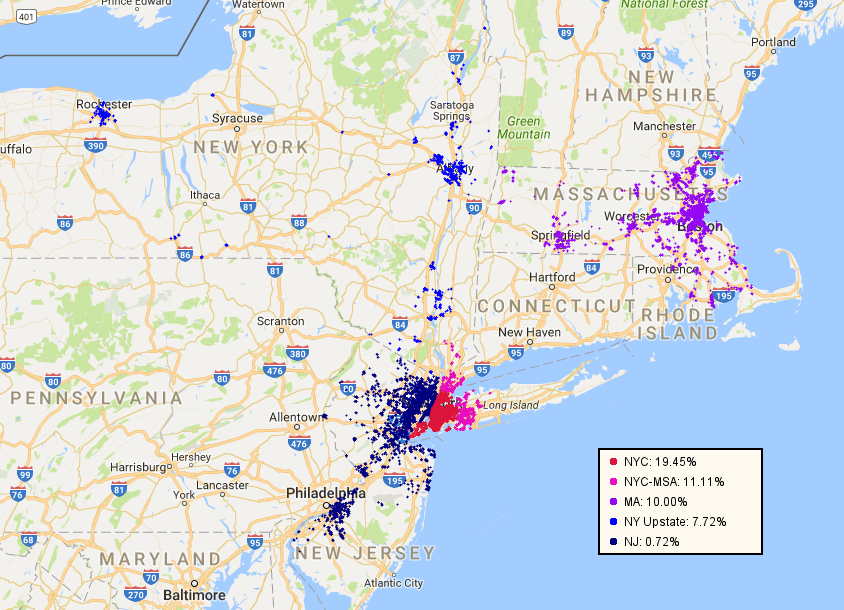
\includegraphics[width=6in]{full_yelp_map.png}

{\footnotesize \raggedright \underline{Notes:} Each data point represents a restaurant in the Yelp dataset. Samples are color coded by the magnitude of the increase in minimum wage on January 1, 2017. NYC saw the highest increase in minimum wage at 19.45\%. NYC-MSA, which includes Nassau, Suffolk, and Westchester counties, saw the second highest increase at 11.11\%. The minimum wage increased in MA by 10.00\%, in Upstate NY by 7.72\% and in NJ by 0.72\%. \par}
\end{figure}

\vspace*{\fill}


\newpage

\vspace*{\fill}


\begin{figure}[H]
\centering
\caption{Geographic Location of Restuarants Used in Border Effects Analysis}
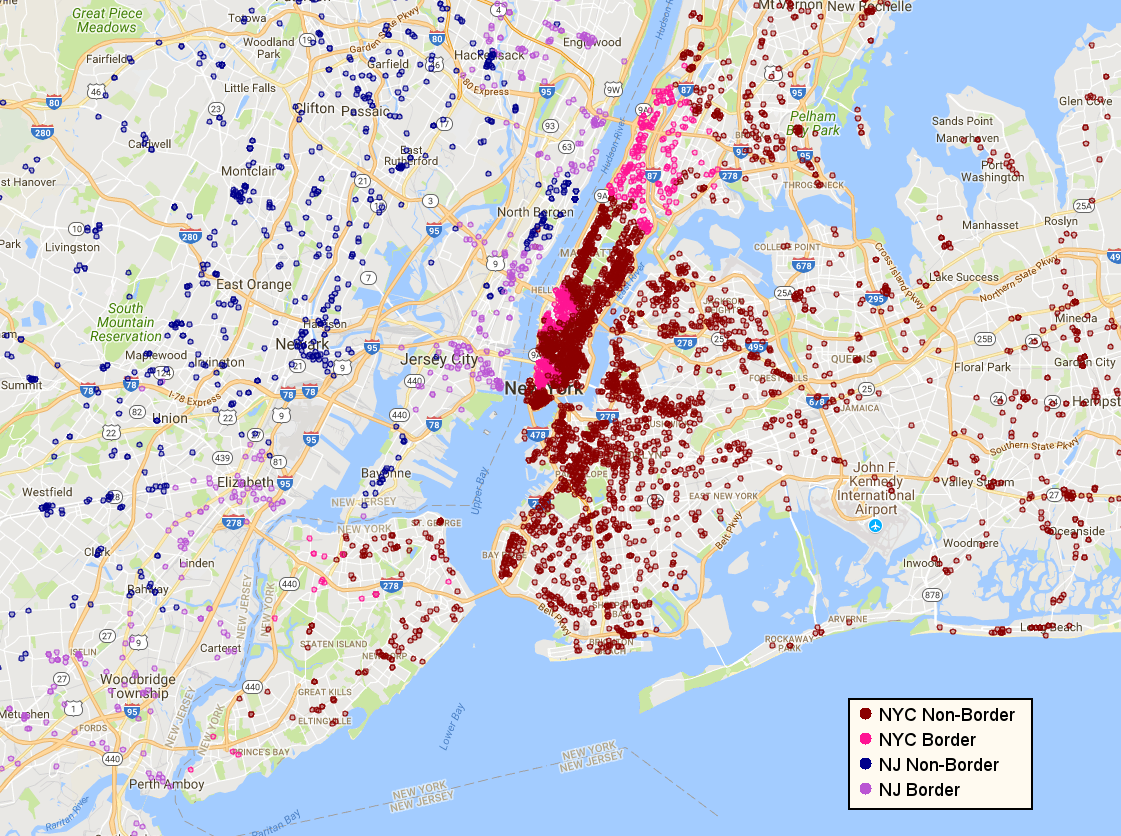
\includegraphics[width=6in]{border.png}

{\footnotesize \raggedright \underline{Notes:} Each data point represents a restaurant in the Yelp dataset in NJ and NYC. Samples are color coded by the magnitude of the increase in minimum wage on January 1, 2017, and use in the border effects analysis. The highlighted restaurants in each group represent the restaurants that are within twelve minutes from the border and are used in the border effects analysis. \par
}
\end{figure}

\vspace*{\fill}

\newpage

\vspace*{\fill}


\begin{figure}[H]
\centering
\caption{Quality Changes by Initial Quality Rating}
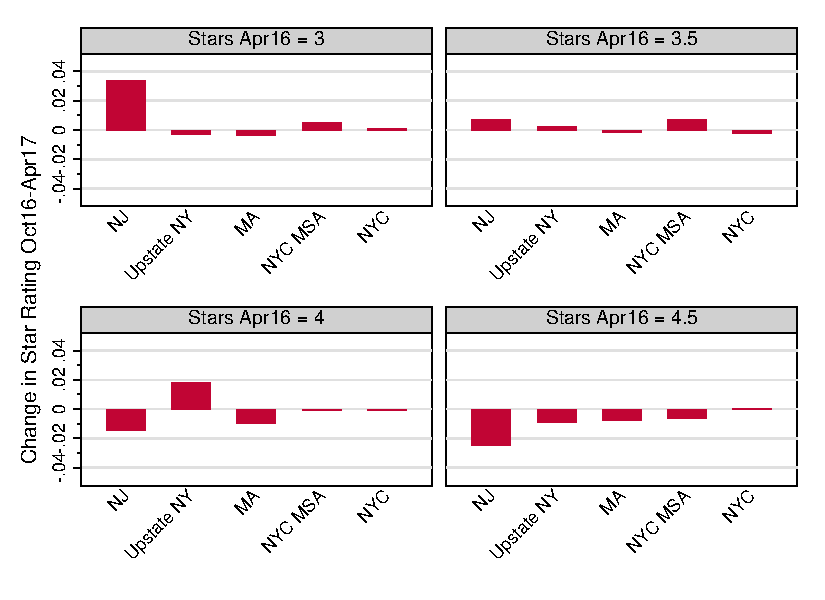
\includegraphics[width=5in]{qualitybars.pdf}

{\footnotesize \raggedright \underline{Notes:} The figures show the relationship between the change in star rating from October 2016 to April 2017 and the change in minimum wage by initial quality rating. The minimum wage groups are reported in ascending order with respect to the increase in minimum wage that occurred in January 2017. The initial star value is the Yelp consumer rating of the restaurants in April 2016. Change in star rating is reported as percentage change. All restaurants that have a star rating throughout the dataset are included in the plots.   \par}
\end{figure}


\vspace*{\fill}


\newpage

\vspace*{\fill}


\begin{figure}[H]
\centering
\caption{Border Effects:  Price Pass Through by Distance to NYC/NJ Border}
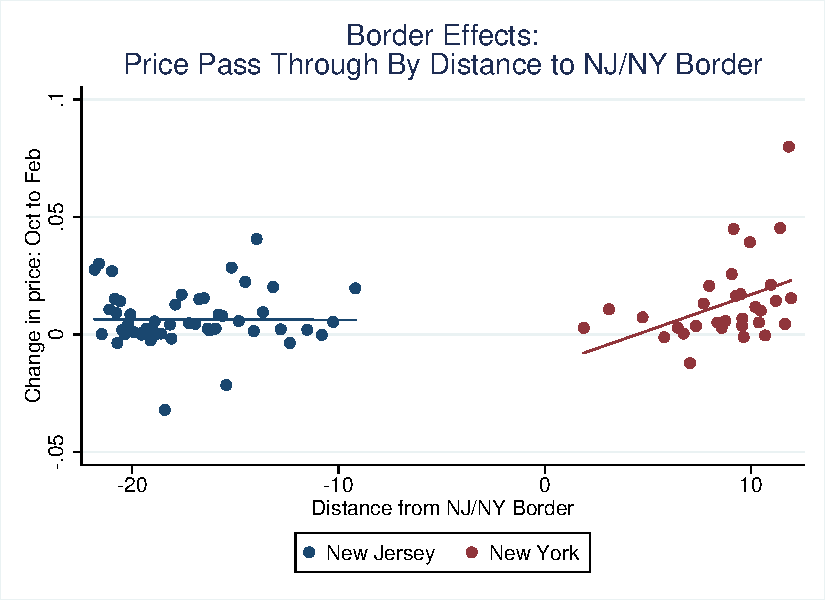
\includegraphics[scale=.75]{gh_dist.pdf}

{\footnotesize \raggedright \underline{Notes:} The figure shows the relationship between the change in price from October 2016 to April 2017 and the distance to the NYC- NJ border. Restaurants are binned into 80 quantiles. There is a gap between the NYC and NJ restaurants due to the Hudson River which separates the two states. Distance is measured in driving minutes to the nearest restaurant on the opposite side of the border. \par }

\end{figure}
%

\vspace*{\fill}


\newpage 

\section{Tables}

\vspace*{\fill}


\begin{table}[H]
\centering
\caption{Minimum Wage Policy Changes}
\begin{tabularx}{1\textwidth}{ l*{1}{Y} c *{6}{Y} } \\ \hline 
%\begin{tabular}{ cccccc } \\ \hline 
 & \multicolumn{3}{c}{Regular Minimum Wage} & \multicolumn{3}{c}{Tipped Minimum Wage}\\
 Area & `16  & `17  & $\% \Delta$ & `16 & `17 &  $\% \Delta$  \\ \hline 
%&&& \\
%1 &  NYC \& FF & \$10.50 & \$12.00 & 14.29\%& - & - & - \\
 %2 & NY Upstate \& FF  & \$9.75 & \$10.75 & 10.26\% & - & -& - \\
 NYC \& Lg & \$9.00 & \$11.00 & 22.22\% & \$7.50 & \$7.50 & 0.00\%\\
 NYC \& Sm & \$9.00 & \$10.50 & 16.67 \% & \$7.50 & \$7.50 & 0.00\%\\
 NYC MSA & \$9.00 & \$10.00 & 11.11\% & \$7.50 & \$7.50 & 0.00\%\\
NY Upstate & \$9.00 & \$9.70 & 7.78\% & \$7.50 & \$7.50  & 0.00\% \\
%7 & Connecticut & \$9.60 & \$10.10 & 5.21\% & \$6.07 & \$6.38 & 5.11\% \\
 New Jersey &  \$8.38 & \$8.44 & 0.72\%  & \$2.13 & \$2.3 & 0.00\% \\
 Massachusetts & \$10.00 & \$11.00 & 10.00\% & \$3.00 & \$3.75  & 25.00\% \\ \hline
%10 & Pennsylvania &  \$7.25 & \$7.25 & 0.00\% & \$2.83 & \$2.83 & 0.00\% \\
%11 & Vermont &  \$9.60 & \$10.00 & 4.2\% & \$4.80 & \$5.00 & 4.2\% \\
\end{tabularx}
%\end{tabular}

\bigskip


{\footnotesize \raggedright \underline{Notes:} The regular and tipped minimum wage changes from 2016 to 2017 are reported by group. The first two rows show the minimum wage changes for restaurants in NYC. A small restaurant is defined as having 10 employees or less, and a large restaurant is defined by more than 10 employees. For the main analysis I use the average of the two minimum wage changes, 19.45\%, for both small and large restaurants in NYC. The NYC MSA group consists of restaurants in the three contiguous counties to NYC: Nassau, Suffolk, and Westchester. NY Upstate encapsulates restaurants in all other areas of the state. NJ and MA minimum wage laws are consistent throughout each state.  \par }
\end{table}

\vspace*{\fill}



\begin{table}[p]
\centering
\caption{Yelp Restaurant Summary Statistics by Minimum Wage Group}
\begin{center}
\begin{tabular}{lccccc}
\hline  & (1) & (2) & (3) & (4) & (5)\\
 & NYC & NYC MSA & MA & NY Upstate & NJ\\
\hline  \textit{Min Wage Increase}  & 0.194 & 0.111 & 0.100 & 0.078 & 0.007\\
  & (0.000) & (0.000) & (0.000) & (0.000) & (0.000)\\
 \textit{Starting Price (Apr16)}  & 9.781 & 10.703 & 9.891 & 9.622 & 9.869\\
  & (7.030) & (6.545) & (5.541) & (8.544) & (7.737)\\
 \textit{Number of Items}  & 60.462 & 78.084 & 67.136 & 62.193 & 73.419\\
  & (80.136) & (82.284) & (76.173) & (72.106) & (90.365)\\
 \textit{Change Price (Apr16-Oct16)}  & 0.005 & 0.002 & 0.003 & 0.003 & 0.005\\
  & (0.048) & (0.060) & (0.057) & (0.033) & (0.044)\\
 \textit{Change Price (Oct16-Apr17)}  & 0.008 & 0.007 & 0.005 & 0.001 & 0.004\\
  & (0.070) & (0.088) & (0.053) & (0.019) & (0.073)\\
 \textit{Increase}  & 0.145 & 0.089 & 0.115 & 0.040 & 0.085\\
  & (0.353) & (0.285) & (0.319) & (0.197) & (0.280)\\
 \textit{Decrease}  & 0.041 & 0.025 & 0.028 & 0.015 & 0.032\\
  & (0.199) & (0.157) & (0.164) & (0.123) & (0.177)\\
 \textit{Price Change $\|$ Increase}  & 0.083 & 0.108 & 0.064 & 0.048 & 0.087\\
  & (0.110) & (0.260) & (0.125) & (0.065) & (0.215)\\
 \textit{Price Change $\|$ Decrease}  & -0.100 & -0.089 & -0.097 & -0.048 & -0.095\\
  & (0.210) & (0.157) & (0.100) & (0.063) & (0.118)\\
 \textit{Sales (100k)}  & 8.489 & 7.597 & 9.233 & 5.019 & 5.631\\
  & (14.245) & (37.176) & (19.165) & (5.988) & (9.583)\\
 \textit{Employees} & 10.836 & 10.227 & 14.603 & 10.222 & 9.267\\
  & (15.415) & (20.926) & (24.594) & (11.832) & (15.260)\\
 \textit{Limited Service}  & 0.042 & 0.072 & 0.019 & 0.069 & 0.043\\
  & (0.201) & (0.258) & (0.135) & (0.254) & (0.202)\\
 \textit{Franchise}  & 0.001 & 0.006 & 0.016 & 0.000 & 0.010\\
  & (0.029) & (0.077) & (0.126) & (0.000) & (0.097)\\
\hline  $ N $  & 4242 & 595 & 1658 & 519 & 1793\\
\hline\end{tabular}\\
\end{center}

{\footnotesize \raggedright \underline{Notes:} The means and standard deviations of the primary dataset, Yelp, are reported. Each column contains the restaurants that fall into a specific minimum wage group. All data is balanced at the item level across time periods and aggregated at the restaurant level. The fourth and fifth rows report mean change in natural log of the price, which is approximately the percentage change. The rows titled ``Increase'' and ``Decrease'' report the percentage of restaurants that increased or decreased price between Oct `16 and Apr '17. The conditional price changes are calculated from Oct `16 to Apr '17. \par }
\end{table}





\begin{table}[p]
\centering
\caption{Grubhub Restaurant Summary Statistics by Minimum Wage Group}
\begin{center}
\begin{tabular}{lccccc}
\hline  & (1) & (2) & (3) & (4) & (5)\\
 & NYC & NYC MSA & MA & NY Upstate & NJ\\
\hline  \textit{Min Wage Increase}  & 0.194 & 0.111 & 0.100 & 0.078 & 0.007\\
  & (0.000) & (0.000) & (0.000) & (0.000) & (0.000)\\
 \textit{Starting Price (Dec16)}  & 9.356 & 9.759 & 9.346 & 8.640 & 8.949\\
  & (5.589) & (3.513) & (4.182) & (2.787) & (3.761)\\
 \textit{Number of Items}  & 107.790 & 133.704 & 117.472 & 105.053 & 126.917\\
  & (89.516) & (87.262) & (73.827) & (74.815) & (87.014)\\
 \textit{Change Price (Dec16-Apr17)}  & 0.013 & 0.008 & 0.009 & 0.013 & 0.006\\
  & (0.044) & (0.027) & (0.036) & (0.036) & (0.034)\\
 \textit{Increase}  & 0.374 & 0.326 & 0.294 & 0.349 & 0.292\\
  & (0.484) & (0.469) & (0.456) & (0.477) & (0.455)\\
 \textit{Decrease}  & 0.066 & 0.060 & 0.053 & 0.047 & 0.073\\
  & (0.249) & (0.238) & (0.224) & (0.213) & (0.260)\\
 \textit{Price Change $\|$ Increase}  & 0.040 & 0.027 & 0.035 & 0.037 & 0.029\\
  & (0.054) & (0.034) & (0.049) & (0.051) & (0.041)\\
 \textit{Price Change $\|$ Decrease}  & -0.025 & -0.019 & -0.030 & -0.011 & -0.026\\
  & (0.076) & (0.054) & (0.068) & (0.019) & (0.075)\\
 \textit{Sales (100k)}  & 8.643 & 3.218 & 4.976 & 4.684 & 2.987\\
  & (42.233) & (4.072) & (7.722) & (6.363) & (3.007)\\
 \textit{Employees} & 9.916 & 5.650 & 7.996 & 9.582 & 5.130\\
  & (18.763) & (7.000) & (12.253) & (13.502) & (5.172)\\
 \textit{Limited Service}  & 0.042 & 0.070 & 0.029 & 0.067 & 0.065\\
  & (0.202) & (0.255) & (0.168) & (0.251) & (0.247)\\
 \textit{Franchise}  & 0.004 & 0.007 & 0.011 & 0.021 & 0.000\\
  & (0.064) & (0.083) & (0.105) & (0.142) & (0.000)\\
\hline  $ N $  & 4172 & 565 & 866 & 358 & 1320\\
\hline\end{tabular}\\
\end{center}

{\footnotesize \raggedright \underline{Notes:}  The means of the secondary dataset, Grubhub, are reported.  Each column contains the restaurants that fall into a specific minimum wage group. All data is balanced at the item level across time periods and aggregated at the restaurant level. The fourth row reports mean change in natural log of the price, which is approximately the percentage change. The rows titled ``Increase'' and ``Decrease'' report the percentage of restaurants that increased or decreased the averaged menu item price between Dec `16 and Apr `17. The conditional price changes calculated from Dec `16 to Apr `17. \par
}
\end{table}



\newpage

%\begin{landscape}
\begin{table}
\centering
\caption{Main Price Pass Through Results}
<<<<<<< HEAD
\begin{center}
\begin{tabular}{lccccc}
\hline  & \multicolumn{3}{c}{Yelp} & \multicolumn{2}{c}{Grubhub}\\
 & (1) & (2) & (3) & (4) & (5)\\
 & All & Cntrls & Change & All & Cntrls\\
\hline  $ Apr16-Jul16 $  & -0.019 & 0.053 & -0.149 &  & \\
 & (0.062) & (0.114) & (0.374) &  & \\
 $ Jul16-Oct16 $  & 0.069 & 0.063 & 0.262 &  & \\
 & (0.080) & (0.120) & (0.409) &  & \\
 $ Oct16-Jan17 $  & 0.163 & 0.208 & 0.604 &  & \\
 & (0.056) & (0.083) & (0.317) &  & \\
 $ Jan17-Apr17 $  & 0.150 & 0.180 & 0.464 &  & \\
 & (0.060) & (0.096) & (0.353) &  & \\
\hline  $ Dec16-Jan17 $  &  &  &  & 0.254 & 0.272\\
 &  &  &  & (0.002) & (0.010)\\
 $ Jan17-Feb17 $  &  &  &  & 0.233 & 0.331\\
 &  &  &  & (0.016) & (0.040)\\
 $ Feb17-Mar17 $  &  &  &  & 0.188 & 0.246\\
 &  &  &  & (0.021) & (0.015)\\
 $ Mar17-Apr17 $  &  &  &  & 0.171 & 0.165\\
 &  &  &  & (0.008) & (0.020)\\
\hline \textit{Total Pass Through} & 0.313 & 0.388 & 1.068 & 0.845 & 1.015$^+$\\
  & (0.115) & (0.171) & (0.669) & (0.031) & (0.083)\\
\hline  $ N $  & 8805 & 5257 & 2099 & 7280 & 3230\\
 $ NxT $  & 35220 & 21028 & 8396 & 29120 & 12920\\
\hline\end{tabular}\\
\begin{tiny}+ statistically different than respective 'All' column \end{tiny}\\
\end{center}
=======
\begin{center}
\begin{tabular}{lccccc}
\hline  & \multicolumn{3}{c}{Yelp} & \multicolumn{2}{c}{Grubhub}\\
 & (1) & (2) & (3) & (4) & (5)\\
 & All & Cntrls & Change & All & Cntrls\\
\hline  $ Apr16-Jul16 $  & -0.019 & 0.053 & -0.149 &  & \\
 & (0.062) & (0.114) & (0.374) &  & \\
 $ Jul16-Oct16 $  & 0.069 & 0.063 & 0.262 &  & \\
 & (0.080) & (0.120) & (0.409) &  & \\
 $ Oct16-Jan17 $  & 0.163 & 0.208 & 0.604 &  & \\
 & (0.056) & (0.083) & (0.317) &  & \\
 $ Jan17-Apr17 $  & 0.150 & 0.180 & 0.464 &  & \\
 & (0.060) & (0.096) & (0.353) &  & \\
\hline  $ Dec16-Jan17 $  &  &  &  & 0.254 & 0.272\\
 &  &  &  & (0.002) & (0.010)\\
 $ Jan17-Feb17 $  &  &  &  & 0.233 & 0.331\\
 &  &  &  & (0.016) & (0.040)\\
 $ Feb17-Mar17 $  &  &  &  & 0.188 & 0.246\\
 &  &  &  & (0.021) & (0.015)\\
 $ Mar17-Apr17 $  &  &  &  & 0.171 & 0.165\\
 &  &  &  & (0.008) & (0.020)\\
\hline \textit{Total Pass Through} & 0.313 & 0.388 & 1.068 & 0.845 & 1.015$^+$\\
  & (0.115) & (0.171) & (0.669) & (0.031) & (0.083)\\
\hline  $ N $  & 8805 & 5257 & 2099 & 7280 & 3230\\
 $ NxT $  & 35220 & 21028 & 8396 & 29120 & 12920\\
\hline\end{tabular}\\
\begin{tiny}+ statistically different than respective 'All' column \end{tiny}\\
\end{center}
>>>>>>> 9bf80c4d3367c601bceb3268e37dc31cf9116a6c


{\footnotesize \raggedright \underline{Notes:}  
The outcome variable for all columns is the log change in price at the restaurant level. All standard errors are clustered at the minimum wage group level. Each row represents the amount of pass-through occurring in the lag(s), lead(s), and contemporaneous time periods of the minimum wage changes. For the specifications using the Yelp data, (1)-(3), the total pass-through estimates are linear combinations of the October '16 to January '17 and the January '17 to April '17 estimates. For the specifications using the Grubhub data, (4)-(5), all time periods are included in the total pass-through estimates. The first column includes the full Yelp sample. The second column includes the vector of controls from the RUSA dataset, comprised of sales volume, number of employees and limited service status. The third column includes only restaurants that changed at least one item over the time period of the dataset. Column 4 reports price pass-through estimates using the full Grubhub sample. Column 5 includes the vector of RUSA control variables.   \par
}
\end{table}
%\end{landscape}



\begin{table}
\centering
\caption{Price Pass Through By Restaurant Characteristics}
\begin{center}
\begin{tabular}{lcccccc}
\hline  & (1) & (2) & (3) & (4) & (5) & (6)\\
 & Low Sales & High Sales & Low Emps & High Emps & Low Stars & High Stars\\
\hline  $ Apr16-Jul16 $  & 0.288 & 0.182 & 0.249 & 0.122 & 0.189 & 0.026\\
 & (0.145) & (0.271) & (0.147) & (0.260) & (0.076) & (0.114)\\
 $ Jul16-Oct16 $  & 0.249 & -0.073 & 0.286 & 0.019 & 0.260 & 0.153\\
 & (0.182) & (0.204) & (0.140) & (0.245) & (0.056) & (0.126)\\
 $ Oct16-Jan17 $  & 0.260 & 0.096 & 0.364 & 0.032 & 0.429 & 0.189\\
 & (0.126) & (0.121) & (0.119) & (0.155) & (0.033) & (0.080)\\
 $ Jan16-Apr17 $  & 0.468 & 0.334 & 0.238 & 0.386 & 0.361 & 0.190\\
 & (0.122) & (0.142) & (0.132) & (0.176) & (0.094) & (0.103)\\
\hline \textit{Total Pass Through} & 0.728 & 0.43 & 0.602$^+$ & 0.418$^+$ & 0.79 & 0.379\\
  & (0.244) & (0.262) & (0.231) & (0.331) & (0.119) & (0.183)\\
\hline  $ N $  & 1556 & 1723 & 2142 & 1894 & 3832 & 6783\\
 $ NxT $  & 6224 & 6892 & 8568 & 7576 & 15328 & 27132\\
\hline\end{tabular}\\
\begin{tiny} + statistically different than comparison group \end{tiny}\\
\end{center}

{\footnotesize \raggedright \underline{Notes:} 
The reported values compare price pass-through of restaurants in the lowest and highest third based on sales, employees, and number of stars in April 2016 using the Yelp dataset. The outcome variable for all columns is the log change in price at the restaurant level. All standard errors are clustered at the minimum wage group level. The total pass-through estimates are linear combinations of the October '16 to January '17 and the January '17 to April '17 estimates.  The cutoff values for sales are 204 and 598 thousand. The cutoff values for employees are 4 and 10, and the cutoff values for stars are 3 and 4. \par
}
\end{table}

\begin{landscape}
\begin{table}
\centering
\caption{Price Pass Through By Item Type}
\begin{center}
\begin{tabular}{lcccccccc}
\hline  & (1) & (2) & (3) & (4) & (5) & (6) & (7) & (8)\\
 & All & Popular & Side & Sandwich & Soup/Salad & Entre & Dessert & Drink\\
\hline  $ Dec16-Jan17 $  & 0.155 & 0.193 & 0.169 & 0.224 & 0.174 & 0.117 & 0.114 & 0.146\\
 & (0.004) & (0.002) & (0.008) & (0.004) & (0.002) & (0.002) & (0.009) & (0.005)\\
 $ Jan17-Feb17 $  & 0.142 & 0.238 & 0.163 & 0.244 & 0.132 & 0.121 & 0.078 & 0.152\\
 & (0.013) & (0.007) & (0.054) & (0.008) & (0.008) & (0.007) & (0.024) & (0.027)\\
 $ Feb17-Mar17 $  & 0.126 & 0.072 & 0.208 & 0.180 & 0.109 & 0.087 & 0.141 & 0.067\\
 & (0.010) & (0.015) & (0.029) & (0.005) & (0.009) & (0.009) & (0.021) & (0.023)\\
 $ Mar17-Apr17 $  & 0.060 & 0.084 & 0.115 & 0.070 & 0.099 & 0.050 & 0.041 & 0.015\\
 & (0.012) & (0.010) & (0.028) & (0.038) & (0.015) & (0.015) & (0.024) & (0.014)\\
\hline \textit{Total Pass Through} & 0.483 & 0.587$^+$ & 0.656$^+$ & 0.718$^+$ & 0.514 & 0.375$^+$ & 0.373 & 0.379$^+$\\
  & (0.032) & (0.023) & (0.104) & (0.045) & (0.022) & (0.026) & (0.076) & (0.054)\\
\hline  $ N $  & 831763 & 47295 & 107172 & 105265 & 46692 & 150035 & 18453 & 65112\\
 $ NxT $  & 3327052 & 189180 & 428688 & 421060 & 186768 & 600140 & 73812 & 260448\\
\hline\end{tabular}\\
\begin{tiny} + statistically different than column (1)\end{tiny}\\
\end{center}

{\footnotesize \raggedright \underline{Notes:} 
The outcome variable for all columns is the log change in price at the item level using the Grubhub dataset. All standard errors are clustered at the minimum wage group level. All time periods are included in the total pass-through estimates. The item categories listed above are mutually exclusive but not exhaustive. The additional food categories not listed include; Appetizer, Kids, Pizza, and Other. \par
}
\end{table}
\end{landscape}

\newpage 

\vspace*{\fill}
%\begin{landscape}
\begin{table}[H]
\centering
\caption{Overall Yelp Quality Changes by Initial Star Rating}
<<<<<<< HEAD
\begin{center}
\begin{tabular}{lcccccc}
\hline  & (1) & (2) & (3) & (4) & (5) & (6)\\
 & All &  $ 2.5 $  &  $ 3.0 $  &  $ 3.5 $  &  $ 4.0 $  &  $ 4.5$ \\
\hline  $ Apr16-Jul16 $  & 0.035 & 1.138 & 0.625 & 0.068 & -1.047 & -0.627\\
 & (0.213) & (1.201) & (0.697) & (0.187) & (0.312) & (0.456)\\
 $ Jul16-Oct16 $  & -0.046 & -0.321 & -0.305 & 0.109 & 0.198 & -0.792\\
 & (0.071) & (0.292) & (0.400) & (0.211) & (0.296) & (0.413)\\
 $ Oct16-Jan17 $  & 0.049 & 0.255 & -1.341 & -0.268 & 0.500 & 0.470\\
 & (0.036) & (1.068) & (0.178) & (0.076) & (0.090) & (0.275)\\
 $ Jan17-Apr17 $  & -0.416 & -1.158 & -0.546 & -0.728 & -0.252 & -0.255\\
 & (0.167) & (0.609) & (0.670) & (0.197) & (0.080) & (0.175)\\
\hline \textit{Total \% Change Stars} & -0.368 & -0.903 & -1.887 & -0.996 & 0.248 & 0.215\\
  & (0.138) & (1.667) & (0.813) & (0.161) & (0.123) & (0.164)\\
\hline  $ N $  & 6392 & 625 & 1080 & 1801 & 1904 & 982\\
 $ NxT $  & 25568 & 2500 & 4320 & 7204 & 7616 & 3928\\
\hline\end{tabular}\\
\begin{tiny} \hfil\end{tiny}\\
\end{center}
=======
\begin{center}
\begin{tabular}{lcccccc}
\hline  & (1) & (2) & (3) & (4) & (5) & (6)\\
 & All &  $ 2.5 $  &  $ 3.0 $  &  $ 3.5 $  &  $ 4.0 $  &  $ 4.5$ \\
\hline  $ Apr16-Jul16 $  & 0.035 & 1.138 & 0.625 & 0.068 & -1.047 & -0.627\\
 & (0.213) & (1.201) & (0.697) & (0.187) & (0.312) & (0.456)\\
 $ Jul16-Oct16 $  & -0.046 & -0.321 & -0.305 & 0.109 & 0.198 & -0.792\\
 & (0.071) & (0.292) & (0.400) & (0.211) & (0.296) & (0.413)\\
 $ Oct16-Jan17 $  & 0.049 & 0.255 & -1.341 & -0.268 & 0.500 & 0.470\\
 & (0.036) & (1.068) & (0.178) & (0.076) & (0.090) & (0.275)\\
 $ Jan17-Apr17 $  & -0.416 & -1.158 & -0.546 & -0.728 & -0.252 & -0.255\\
 & (0.167) & (0.609) & (0.670) & (0.197) & (0.080) & (0.175)\\
\hline \textit{Total \% Change Stars} & -0.368 & -0.903 & -1.887 & -0.996 & 0.248 & 0.215\\
  & (0.138) & (1.667) & (0.813) & (0.161) & (0.123) & (0.164)\\
\hline  $ N $  & 6392 & 625 & 1080 & 1801 & 1904 & 982\\
 $ NxT $  & 25568 & 2500 & 4320 & 7204 & 7616 & 3928\\
\hline\end{tabular}\\
\begin{tiny} \hfil\end{tiny}\\
\end{center}
>>>>>>> 9bf80c4d3367c601bceb3268e37dc31cf9116a6c

{\footnotesize \raggedright \underline{Notes:} 
The outcome variable for all columns is the log change in Yelp star rating. All standard errors are clustered at the minimum wage group level. The total percent change in stars estimates are linear combinations of the October '16 to January '17 and the January '17 to April '17 estimates. The initial star ratings are the rounded Yelp star ratings in April '16. Restaurants below a 2.5 rating and above a 4.5 rating are not analyzed as subsamples given that they are close to the lower and upper bounds, respectively, and so only have one direction to move. \par
}
\end{table}
%\end{landscape}
\vspace*{\fill}

\newpage 

\vspace*{\fill}

\begin{table}[H]\caption{Grubhub Food Specific Quality Changes by Initial Quality Rating}
<<<<<<< HEAD
\begin{center}
\begin{tabular}{lccc}
\hline  & (1) & (2) & (3)\\
 & All &  $<=$ Median  &  $>$ Median\\
\hline  $ Dec16-Jan17 $  & -0.069 & -0.349 & 0.156\\
 & (0.061) & (0.181) & (0.052)\\
 $ Jan17-Feb17 $  & -0.023 & -0.210 & 0.136\\
 & (0.102) & (0.169) & (0.049)\\
 $ Feb17-Mar17 $  & -0.171 & -0.317 & -0.018\\
 & (0.045) & (0.051) & (0.037)\\
 $ Mar17-Apr17 $  & -0.054 & -0.176 & 0.048\\
 & (0.019) & (0.056) & (0.066)\\
\hline \textit{Total \% Change Rating} & -0.316 & -1.215 & 0.344\\
  & (0.000) & (0.003) & (0.004)\\
\hline  $ N $  & 7281 & 3979 & 3302\\
 $ NxT $  & 29124 & 15916 & 13208\\
\hline\end{tabular}\\
\begin{tiny} \hfil\end{tiny}\\
\end{center}
=======
\begin{center}
\begin{tabular}{lccc}
\hline  & (1) & (2) & (3)\\
 & All &  $<=$ Median  &  $>$ Median\\
\hline  $ Dec16-Jan17 $  & -0.069 & -0.349 & 0.156\\
 & (0.061) & (0.181) & (0.052)\\
 $ Jan17-Feb17 $  & -0.023 & -0.210 & 0.136\\
 & (0.102) & (0.169) & (0.049)\\
 $ Feb17-Mar17 $  & -0.171 & -0.317 & -0.018\\
 & (0.045) & (0.051) & (0.037)\\
 $ Mar17-Apr17 $  & -0.054 & -0.176 & 0.048\\
 & (0.019) & (0.056) & (0.066)\\
\hline \textit{Total \% Change Rating} & -0.316 & -1.215 & 0.344\\
  & (0.000) & (0.003) & (0.004)\\
\hline  $ N $  & 7281 & 3979 & 3302\\
 $ NxT $  & 29124 & 15916 & 13208\\
\hline\end{tabular}\\
\begin{tiny} \hfil\end{tiny}\\
\end{center}
>>>>>>> 9bf80c4d3367c601bceb3268e37dc31cf9116a6c

{\footnotesize \raggedright \underline{Notes:} 
The outcome variable for all columns is the log change in Grubhub Food Quality rating. The food specific quality rating is on a 1 to 100 scale and represents the proportion of customers that reported that ``the food was good" after receiving their order. All standard errors are clustered at the minimum wage group level. The total percent change in rating estimates are linear combinations of all rows. The median food quality rating is 89. \par
}
\end{table}

\vspace*{\fill}


\vspace*{\fill}

% \vspace{100mm} 

\newpage 

\vspace*{\fill}
\begin{table}[H]
\centering
\caption{Border Effects}
\begin{center}
\begin{tabular}{lccc}
\hline Source & \multicolumn{2}{c}{Yelp} & Grubhub\\
 & (1) & (2) & (3)\\
Time Frame & Oct16-Apr17 & Apr16-Oct16 & Dec16-Apr17\\
\hline  $ \mathbbm{1}(NY) \quad (\alpha_1) $  & 0.0064 & -0.0064 & -0.0102\\
  & (0.0152) & (0.0116) & (0.0124)\\
 Distance $\quad (\alpha_2) $  & -0.0009 & 0.0000 & -0.0000\\
  & (0.0008) & (0.0006) & (0.0006)\\
 Distance * $ \mathbbm{1}(NY) \quad (\alpha_3) $  & 0.0020 & 0.0007 & 0.0019\\
  & (0.0011) & (0.0009) & (0.0009)\\
 Constant $\quad (\alpha_0) $  & -0.0069 & 0.0041 & 0.0059\\
  & (0.0134) & (0.0102) & (0.0101)\\
\hline  $ \alpha_2 + \alpha_3 $  & 0.0011 & 0.0007 & 0.0018\\
  & (0.0008) & (0.0006) & (0.0007)\\
\hline  $ N $  & 1002 & 1002 & 694\\
\hline\end{tabular}\\
\end{center}

{\footnotesize \raggedright \underline{Notes:} 
The outcome variable is the percentage point change in price due to a 10 minute change in the distance of a restaurant to the border. The first column includes restaurants in the Yelp dataset within twelve minutes of the NYC - NJ border between October 2016 and April 2017. Column 2 includes these same restaurants but using the change in price from July 2016 to October 2016 as the outcome. Column 3 reports effects on the NYC-NJ border using the Grubhub dataset. \par
}
\end{table}
\vspace*{\fill}

%
%\section{Appendix}
%
%\subsection{Data Collection}
%
%\subsection{Variable Definitions}
%






\end{document}












>>>>>>> 9bf80c4d3367c601bceb3268e37dc31cf9116a6c
